% !TeX spellcheck = es_ES

%----------------------------------------------------------------------------------------



\part{Capítulo tres}
\graphicspath{ {3_Capitulo/img/ejemplos/} {img/ch3/}, {W_Varios/2_Portada_capitulos} }

%----------------------------------------------------------------------------------------
%	CHAPTER 3
%----------------------------------------------------------------------------------------

\chapterimage{3_Capitulo/img/portada/ima2} % Chapter heading image
\chapter{Aplicaciones de interés compuesto}

\section{Mapa Mental}
\begin{center}
 \includegraphics[height = 5.6 cm]{3_Capitulo/img/explicacion/"Mapa Mental 3.pdf"}\\
\end{center}
\newpage
\section{Fórmulas del capítulo}
\begin{spacing}{1.5}
 \begin{center}
  \begin{tabular}{ |p{6cm}|p{7cm}| p{2cm}|}
   \hline
   \rowcolor{orange!50}
   \begin{center}\textbf{Fórmula} \end{center}             & \begin{center} \textbf{Nombre}\end{center} & \begin{center} \textbf{Excel} \end{center} \\ \hline
   $i =i_{1} + i_{2} + (i_{1})(  i_{2})$ & Tasas de referencia       & -                         \\ \hline
   $ i = \frac{i-i_{f}}{1+i_{f}} $       & Tasa de interés real      & -                         \\ \hline
  \end{tabular}
 \end{center}
\end{spacing}

\section{Depósito a término fijo}

Un intermediario financiero debe conseguir dinero del público con una tasa de interés que incentive a los inversionistas, esta tasa es llamada tasa de captación, para prestar este dinero con una tasa más alta llamada tasa de colocación.

\subsection{Certificado de depósito a término}
Es el certificado que se recibe por depósitos de sumas de dinero. Los plazos más usados son 30, 60, 90, 180 y 360 días. Pueden emitirlos las entidades financieras. La tasa de interés por su depósito está determinada por el monto, el plazo y las condiciones existentes en el mercado al momento de su constitución. Son nominativos y no se pueden redimir antes de su vencimiento.\\



%%%%%%%%%% NO OLVIDAR COLOCAR ESTE COMENTARIO CON EL NUMERO DE EJERCICIO %%%%%%%%%%%%%
%%%%%%%%%%%%%%%%%%% EJERCICIO 1 %%%%%%
\textbf{Ejemplo 1}\\
Para realizar un proyecto se necesita realizar una inversión inicial de 80.000 COP y otra inversión de
45.000 COP al final del primer mes, en los meses 2 y 3 los ingresos son equivalentes a los egresos;
pero a partir del mes 4, se producen ingresos así: Mes cuatro 30.000 COP, mes cinco 50.000 COP, mes
seis 60.000 COP. Determinar si el proyecto lo pueden realizar los inversionistas A o B mencionados
anteriormente.\\


%%%%%%%%%%%%%%%%%%% EJERCICIO 1 %%%%%%

%\newpage %USAR SOLO SI EL SOLUCION QUEDA SOLO Y ES NECESARIO BAJARLO A LA SIGUIENTE PAGINA
\textbf{Solución.}\\
%La tabla ira centrada
\begin{center}
	\renewcommand{\arraystretch}{1.5}% Margenes de las celdas
	%Creacion de la cuadricula de 3 columnas \end{flushleft}
	\begin{longtable}[H]{|C{0.3\linewidth}|C{0.3\linewidth}|C{0.3\linewidth}|}
		%Creamos una linea horizontal
		\hline
         %%%%% INICIO FLUJO DE CAJA
		\rowcolor[HTML]{FFB183}
		\multicolumn{3}{|c|}{\cellcolor[HTML]{FFB183}\textbf{1. Asignación periodo focal}}   \\ \hline
		\multicolumn{3}{|c|} {$pf = 0 pmv$} \\ \hline
		%%%%%%%%%% FIN TITULO
		%%%%%%%%%% INICIO TITULO
		%Lo que se hace aqui es mezclar las 3 columnas en una sola
		\multicolumn{3}{|c|}{\cellcolor[HTML]{FFB183}\textbf{2. Declaración de variables}}   \\ \hline
		%%%%%%%%%% FIN TITULO
		%%%%%%%%%% INICIO DE MATEMATICAS
		%Cada & hace referencia al paso de la siguiente columna
		$n_{0} = 0 pmv$   & $n_{1} = 1 pmv$ & $n_{2} =  4 pmv$\\
		$n_{3} = 5 pmv$ & $n_{4} = 6 pmv$ & \\ \hline
		\multicolumn{3}{|c|}{$i_{a} = TIO_{a} = 3\% \equiv 0.03 pmv$} \\
		\multicolumn{3}{|c|}{$i_{b} = TIO_{b} = 2\% \equiv 0.02 pmv$} \\ \hline
		%%%%%%%%%% FIN DE MATEMATICAS
		%%%%% FIN DECLARACION DE VARIABLES


		%%%%% INICIO FLUJO DE CAJA
		\rowcolor[HTML]{FFB183}
		\multicolumn{3}{|c|}{\cellcolor[HTML]{FFB183}\textbf{3. Diagrama de flujo de caja}} \\ \hline
		%Mezclamos 3 columnas y ponermos el dibujo
		%%%%%%%%%%%%% INSERCION DE LA IMAGEN
		%Deberan descargar las imagenes respectivas del drive y pegarlas en la carpeta
		%n_capitulo/img/ejemplos/1/capitulo1ejemplo1.pdf  (el /1/ es el numero del ejemplo)
		\multicolumn{3}{|c|}{ 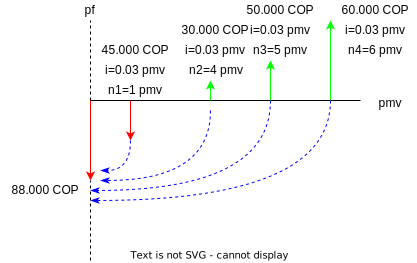
\includegraphics[trim=-5 -5 -5 -5 , scale=1.0,width=300px, height=250px]{9_Capitulo/ejemplos/1/Capitulo9Ejercicio1.pdf} }   \\ \hline
		%%%%%%%%%%%%% FIN INSERCION DE IMAGEN
		%%%%%FIN FLUJO DE CAJA



		%%%%% INICIO DECLARACION FORMULAS
		%%%%%%%%%%% INICIO TITULO
		\rowcolor[HTML]{FFB183}
		\multicolumn{3}{|c|}{\cellcolor[HTML]{FFB183}\textbf{4. Declaración de fórmulas}}    \\ \hline
		%%%%%%%%%%% FIN TITULO
		%%%%%%%%%%% INICIO MATEMATICAS
		\multicolumn{3}{|c|}{$\sum F_{n}(1+i)^{-n} $\hspace{0.3cm} \textit{Valor presente neto}} \\ \hline
		%%%%%%%%%% FIN MATEMATICAS
		%%%%%% INICIO DESARROLLO MATEMATICO
		\rowcolor[HTML]{FFB183}
		%%%%%%%%%%INICIO TITULO
		\multicolumn{3}{|c|}{\cellcolor[HTML]{FFB183}\textbf{5. Desarrollo matemático}}       \\ \hline
		%%%%%%%%%% FIN TITULO
		%%%%%%%%%% INICIO MATEMATICAS
		\multicolumn{3}{|c|}{$VPN_{a} = -80000 - 45000(1+0.03)^{-1} + 30000(1+0.03)^{-4} + 50000(1+0.03)^{-5} + 60000(1+0.03)^{-6}$} \\
		\multicolumn{3}{|c|}{$VPN_{a} = -3655$} \\
		\multicolumn{3}{|c|}{$VPN_{b} = -80000 - 45000(1+0.02)^{-1} + 30000(1+0.02)^{-4} + 50000(1+0.02)^{-5} + 60000(1+0.02)^{-6}$} \\
		\multicolumn{3}{|c|}{$VPN_{b} = 216254$} \\ \hline

		%%%%%%%%%% FIN MATEMATICAS
		%%%%%% FIN DESARROLLO MATEMATICO
		%%%%%% INICIO RESPUESTA
		\rowcolor[HTML]{FFB183}
		%%%%%%%%%%INICIO TITULO
		\multicolumn{3}{|c|}{\cellcolor[HTML]{FFB183}\textbf{6. Respuesta}}   \\ \hline
		%%%%%%%%%% FIN TITULO
		%%%%%%%%%% INICIO RESPUESTA MATEMATICA
		\multicolumn{3}{|c|}{Para B el $VPN > 0$, significa que puede realizar el proyecto en pesos de hoy,} \\ 
		\multicolumn{3}{|c|}{además de ganarse el 2\%, obtiene una ganancia de 2.162,54 COP.}  \\ \hline
		%%%%%%%%%% FIN MATEMATICAS
		%%%%%% FIN RESPUESTA
	\end{longtable}
	%Se crean dos lineas en blanco para que no quede el siguiente texto tan pegado
	%\newline \newline %USARLO SI CREES QUE ES NECESARIO
\end{center}
%%%%%%%%%%%%%%%%%%%%%%%%%%FIN EJERCICIO 1 %%%%%%%%%%%%%%%%%%%%%%%%%%%

%%%%%%%%%%%%%%%%%%%%%%%%%%FIN EJERCICIO 1 %%%%%%%%%%%%%%%%%%%%%%%%%%%


\subsection{Inflación ($i_f$)}
Mide el crecimiento del nivel general de precios de la economía. La inflación es calculada mensualmente por el DANE sobre los precios de una canasta básica de bienes y servicios de consumo para familias de ingresos medios y bajos. Con base en estos precios se calcula un índice denominado Índice de Precios al Consumidor (IPC). La inflación corresponde a la variación periódica de ese índice.\\
La inflación y la deflación son fenómenos internos de un país, la devaluación es externa.

\subsection{Índice}
Mide las variaciones de un fenómeno económico o de otro orden referido a un valor que se toma como base en un momento dado. Relación de precios, de cantidades, de valores entre dos períodos dados.

\subsection{Índice de precios al consumidor (IPC)}
Variación que entre un mes y otro presentan los precios de bienes y servicios de consumo final correspondientes a una canasta típica.

\subsection{Tasa promedio de captaciones Básica de Superfinanciera (TBS)}
Es la tasa promedio de captación a través de CDT y CDAT de las entidades financieras, calculada diariamente por la Superintendencia Financiera para diferentes plazos.

\section{Devaluación (idev)}
La pérdida de valor de una moneda frente a otra moneda se denomina devaluación (pagar  1{.}500 COP por un dólar,  2{.}000 COP un año después). En este caso la devaluación del año es igual a la variación de precio sobre el precio inicial, esto es: \\

devaluación = $\frac{ 2{.}000 \ COP - 1{.}500 \ COP}{ 1{.}500 \ COP} = 0,333333 $ = 33,33\% pav \\

La revaluación significa que habrá que pagar menos pesos por el mismo dólar (pagar  COP 1{.}500 por un dólar,  COP 1{.}200 un año después) entonces la revaluación será variación de precio sobre el precio inicial así: \\

revaluación = $\frac{ 1{.}200 \ COP - 1{.}500 \ COP}{ 1{.}500 \ COP} = -0,2$ = -20\% pav \\

\subsection{LIBOR (London Interbank Offer Rate)}
Tasa de interés anual para los préstamos interbancarios de primera clase en Londres y Europa.
\\
\\
%%%%%%%%%% NO OLVIDAR COLOCAR ESTE COMENTARIO CON EL NUMERO DE EJERCICIO %%%%%%%%%%%%%
%%%%%%%%%%%%%%%%%%% EJERCICIO 2 %%%%%%
\textbf{Ejemplo 2}\\
Se invierten 200{.}000 COP en un depósito a término fijo de 6 meses en un banco que paga el 28\% namv. Determinar el monto de la entrega al vencimiento.\\

%%%%%%%%%%%%%%%%%%% EJERCICIO 1 %%%%%%

%\newpage %USAR SOLO SI EL SOLUCIÓN QUEDA SOLO Y ES NECESARIO BAJARLO A LA SIGUIENTE PAGINA
\textbf{Solución.}
%La tabla ira centrada
\begin{center}
  \renewcommand{\arraystretch}{1.5}% Margenes de las celdas
  %Creación de la cuadricula de 3 columnas \end{flushleft}
  \begin{longtable}[H]{|C{0.3\linewidth}|C{0.3\linewidth}|C{0.3\linewidth}|}
    %Creamos una linea horizontal
    \hline
    %Definimos el color de la primera fila
    \rowcolor[HTML]{FFB183}
    %%%%% INICIO ASIGNACIÓN FECHA FOCAL %%%%%%%
    %%%%%%%%%% INICIO TITULO
    %Lo que se hace aquí es mezclar las 3 columnas en una sola
    \multicolumn{3}{|c|}{\cellcolor[HTML]{FFB183}\textbf{1. Asignación período focal}}                                  \\ \hline
    %%%%%%%%%% FIN TITULO
    %%%%% INICIO DECLARACIÓN DE VARIABLES %%%%%%%
    \multicolumn{3}{|c|}{$pf = 6pmv$}                                                                                   \\ \hline
    %%%%%%%%%% INICIO TITULO
    %Lo que se hace aquí es mezclar las 3 columnas en una sola
    \multicolumn{3}{|c|}{\cellcolor[HTML]{FFB183}\textbf{2. Declaración de variables}}                                  \\ \hline
    %%%%%%%%%% FIN TITULO
    %%%%%%%%%% INICIO DE MATEMÁTICAS
    %Cada & hace referencia al paso de la siguiente columna
    $P =  200{.}000$ COP & $n = 6\textit{pmv} $ & $i= ?\% pmv$                                                           \\
    $j=28\%namv$         & $m=12pmv$            & $F = ? COP$                                                           
    \\\hline

    %%%%%%%%%% FIN DE MATEMÁTICAS
    %%%%% FIN DECLARACIÓN DE VARIABLES


    %%%%% INICIO FLUJO DE CAJA
    \rowcolor[HTML]{FFB183}
    \multicolumn{3}{|c|}{\cellcolor[HTML]{FFB183}\textbf{3. Diagrama de flujo de caja}}                                 \\ \hline
    %Mezclamos 3 columnas y pondremos el dibujo
    %%%%%%%%%%%%% INSERCIÓN DE LA IMAGEN
    %Deberán descargar las imágenes respectivas del drive y pegarlas en la carpeta
    %n_capitulo/img/ejemplos/1/capitulo1ejemplo1.pdf  (el /1/ es el numero del ejemplo)
    \multicolumn{3}{|c|}{ 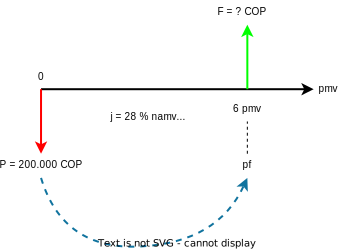
\includegraphics[trim=-5 -5 -5 -5 , scale=1]{2_Capitulo/ejemplos/2/Capitulo2Ejercicio2_v2.pdf} } \\ \hline
    %%%%%%%%%%%%% FIN INSERCIÓN DE IMAGEN
    %%%%%FIN FLUJO DE CAJA



    %%%%% INICIO DECLARACIÓN FORMULAS
    %%%%%%%%%%% INICIO TITULO
    \rowcolor[HTML]{FFB183}
    \multicolumn{3}{|c|}{\cellcolor[HTML]{FFB183}\textbf{4. Declaración de fórmulas}}                                   \\ \hline
    %%%%%%%%%%% FIN TITULO
    %%%%%%%%%%% INICIO MATEMÁTICAS
    \multicolumn{3}{|c|}{$F = P(1+i)^n \hspace{0.3cm} \textit{Valor futuro}$}                                           \\
    \multicolumn{3}{|c|}{$j=i\cdot m\hspace{0.3cm}\textit{Tasa periódica anualizada}$}
    \\ \hline
    %%%%%%%%%% FIN MATEMÁTICAS
    %%%%%% INICIO DESARROLLO MATEMÁTICO
    \rowcolor[HTML]{FFB183}
    %%%%%%%%%%INICIO TITULO
    \multicolumn{3}{|c|}{\cellcolor[HTML]{FFB183}\textbf{5. Desarrollo matemático}}                                     \\ \hline
    %%%%%%%%%% FIN TITULO
    %%%%%%%%%% INICIO MATEMÁTICAS
    \multicolumn{3}{|c|}{$0{.}28=i\cdot 12$}                                                                            \\
    \multicolumn{3}{|c|}{$i= \frac{0{.}28}{12} = 0{.}02333... \equiv 2{.}333\%pmv$}                                     \\
    \multicolumn{3}{|c|}{$0{.}28=i\cdot 12$}                                                                            \\
    \multicolumn{3}{|c|}{$F = 200{.}000 COP(1+0,2333)^6$}                                                       \\
    \multicolumn{3}{|c|}{$F = 229{.}685.04 COP$}
    \\ \hline


    %%%%%%%%%% FIN MATEMÁTICAS
    %%%%%% FIN DESARROLLO MATEMÁTICO
    %%%%%% INICIO RESPUESTA
    \rowcolor[HTML]{FFB183}
    %%%%%%%%%%INICIO TITULO
    \multicolumn{3}{|c|}{\cellcolor[HTML]{FFB183}\textbf{6. Respuesta}}                                                 \\ \hline
    %%%%%%%%%% FIN TITULO
    %%%%%%%%%% INICIO RESPUESTA MATEMÁTICA
    \multicolumn{3}{|c|}{$F = 229{.}685.04 COP$
    }                                                                                                                   \\ \hline
    %%%%%%%%%% FIN MATEMÁTICAS
    %%%%%% FIN RESPUESTA
  \end{longtable}
  %Se crean dos lineas en blanco para que no quede el siguiente texto tan pegado
  %\newline \newline %USARLO SI CREES QUE ES NECESARIO
\end{center}
%%%%%%%%%%%%%%%%%%%%%%%%%%FIN EJERCICIO 1 %%%%%%%%%%%%%%%%%%%%%%%%%%%

%%%%%%%%%%%%%%%%%%%%%%%%%%FIN EJERCICIO 2 %%%%%%%%%%%%%%%%%%%%%%%%%%%


\section{Tasas combinadas}

Cuando se combina una tasa $i_{1}$ con una tasa $i_{2}$, con el objetivo de facilitar los cálculos se puede utilizar la tasa combinada "i". Para este fin se usa la siguiente fórmula:\\
\centerline{$ i = i_{1} +i_{2} + (i_{1})( i_{2})$ \hspace{15pt}\textit{ Tasas combinadas}\\}
\textbf{Nota:} Se utiliza únicamente para el cálculo de tasas de interés anuales, por ejemplo, para calcular la tasa equivalente entre dos tasas efectivas.\\


%%%%%%%%%% NO OLVIDAR COLOCAR ESTE COMENTARIO CON EL NUMERO DE EJERCICIO %%%%%%%%%%%%%
%%%%%%%%%%%%%%%%%%% EJERCICIO 3 %%%%%%
\textbf{Ejemplo 3}\\
Una fabrica produce actualmente en forma manual 1.000 unidades de un determinado artículo, para ello utiliza artesanos a los cuales les paga 8.400.000 COP al año y, es costumbre que cada año se les aumente el sueldo en aproximadamente un 20\%. El precio de venta de cada artículo es de 9.000 COP y se estima que este precio podrá ser aumentado todos los años en un 21\%. Ahora se ha presentado la oportunidad de adquirir una máquina a un costo de 10 millones COP con una vida útil de 5 años; un valor de salvamento de 2 millones COP la cual requiere de 2 técnicos para su operación, el sueldo anual de cada uno de los técnicos puede ser de 600.000 COP con aumentos anuales de sueldo del 20\% ¿Cuál de las dos alternativas es mejor suponiendo que la tasa del inversionista es del 30\%?\\


%%%%%%%%%%%%%%%%%%% EJERCICIO 3 %%%%%%

%\newpage %USAR SOLO SI EL SOLUCION QUEDA SOLO Y ES NECESARIO BAJARLO A LA SIGUIENTE PAGINA
\textbf{Solución.}\\
%La tabla ira centrada
\begin{center}
	\renewcommand{\arraystretch}{1.5}% Margenes de las celdas
	%Creacion de la cuadricula de 3 columnas \end{flushleft}
	\begin{longtable}[H]{|C{0.3\linewidth}|C{0.3\linewidth}|C{0.3\linewidth}|}
		%Creamos una linea horizontal
		\hline
        %%%%% INICIO FLUJO DE CAJA
		\rowcolor[HTML]{FFB183}
		\multicolumn{3}{|c|}{\cellcolor[HTML]{FFB183}\textbf{1. Asignación periodo focal}}   \\ \hline
		\multicolumn{3}{|c|} {$pf = 0 pav$} \\ \hline
		%%%%%%%%%% FIN TITULO
		%%%%%%%%%% INICIO TITULO
		%Lo que se hace aqui es mezclar las 3 columnas en una sola
		\multicolumn{3}{|c|}{\cellcolor[HTML]{FFB183}\textbf{2. Declaración de variables}}   \\ \hline
		%%%%%%%%%% FIN TITULO
		%%%%%%%%%% INICIO DE MATEMATICAS
		%Cada & hace referencia al paso de la siguiente columna
		$R_{1} = 9.000.000 $ COP   & $R_{2} = 8.400.000$ COP  & $i=0.3pav$\\ 
		$g_{1} =  0.21 pav $ & $g_{2}=  0.2 pav $ & $n=5pav$ \\ \hline
		%%%%%%%%%% FIN DE MATEMATICAS
		%%%%% FIN DECLARACION DE VARIABLES

  		%%%%% INICIO DECLARACION FORMULAS
  
		%%%%%%%%%%% INICIO TITULO
		\rowcolor[HTML]{FFB183}
		\multicolumn{3}{|c|}{\cellcolor[HTML]{FFB183}\textbf{3. Diagrama de flujo de caja}} \\ \hline
		%Mezclamos 3 columnas y ponermos el dibujo
		%%%%%%%%%%%%% INSERCION DE LA IMAGEN
		%Deberan descargar las imagenes respectivas del drive y pegarlas en la carpeta
		%n_capitulo/img/ejemplos/1/capitulo1ejemplo1.pdf  (el /1/ es el numero del ejemplo)
		\multicolumn{3}{|c|}{ \includegraphics[trim=-5 -5 -5 -5 , scale=1, width=300px, height=250px]{9_Capitulo/ejemplos/3/Capitulo9Ejercicio3.pdf} }   \\ \hline
		%%%%%%%%%%%%% FIN INSERCION DE IMAGEN
		%%%%%FIN FLUJO DE CAJA



		%%%%% INICIO DECLARACION FORMULAS
		%%%%%%%%%%% INICIO TITULO
		\rowcolor[HTML]{FFB183}
		\multicolumn{3}{|c|}{\cellcolor[HTML]{FFB183}\textbf{4. Declaración de fórmulas}}    \\ \hline
		%%%%%%%%%%% FIN TITULO
		%%%%%%%%%%% INICIO MATEMATICAS
		\multicolumn{3}{|c|}{$\sum F_{n}(1+i)^{-n} $\hspace{0.3cm} \textit{Valor presente neto}} \\ \hline
		%%%%%%%%%% FIN MATEMATICAS
		%%%%%% INICIO DESARROLLO MATEMATICO
		\rowcolor[HTML]{FFB183}
		%%%%%%%%%%INICIO TITULO
		\multicolumn{3}{|c|}{\cellcolor[HTML]{FFB183}\textbf{5. Desarrollo matemático}}       \\ \hline
		%%%%%%%%%% FIN TITULO
		%%%%%%%%%% INICIO MATEMATICAS
		\multicolumn{3}{|c|}{$VPN_{A} = \frac{9[(1+0.21)^{5}(1+0.3)^{-5} -1]}{0.21-0.3} - \frac{8.4[(1+0.2)^{5}(1+0.3^{-5} -1)]}{0.2-0.3}$} \\
		\multicolumn{3}{|c|}{$VPN_{A} = 2.437.836 $ COP} \\
		\multicolumn{3}{|c|}{$VPN_{B} = \frac{9[(1+0.21)^{5}(1+0.3)^{-5} -1]}{0.21-0.3} + 2(1.3)^{-5} - \frac{1.2[(1+0.2)^{5}(1+0.3^{-5} -1)]}{0.2-0.3}$} \\
		\multicolumn{3}{|c|}{$VPN_{B} = 16.723.756 $ COP} \\ \hline

		%%%%%%%%%% FIN MATEMATICAS
		%%%%%% FIN DESARROLLO MATEMATICO
		%%%%%% INICIO RESPUESTA
		\rowcolor[HTML]{FFB183}
		%%%%%%%%%%INICIO TITULO
		\multicolumn{3}{|c|}{\cellcolor[HTML]{FFB183}\textbf{6. Respuesta}}   \\ \hline
		%%%%%%%%%% FIN TITULO
		%%%%%%%%%% INICIO RESPUESTA MATEMATICA
		\multicolumn{3}{|c|}{La decisión correcta es comprar la máquina.}  \\ \hline
		%%%%%%%%%% FIN MATEMATICAS
		%%%%%% FIN RESPUESTA
	\end{longtable}
	%Se crean dos lineas en blanco para que no quede el siguiente texto tan pegado
	%\newline \newline %USARLO SI CREES QUE ES NECESARIO
\end{center}
%%%%%%%%%%%%%%%%%%%%%%%%%%FIN EJERCICIO 3 %%%%%%%%%%%%%%%%%%%%%%%%%%%

%%%%%%%%%%%%%%%%%%%%%%%%%%FIN EJERCICIO 3 %%%%%%%%%%%%%%%%%%%%%%%%%%%



\section{Tasa real}
Para un proyecto de inversión se tiene en cuenta que la inflación afecta la rentabilidad real del proyecto y que siempre se desea obtener una rentabilidad superior a la tasa de oportunidad. Para calcular la rentabilidad real se hace uso de la fórmula asumiendo que la inflación "$i_{1} = i_ {f} $", que la rentabilidad "$i_{2} = i_ {R} $" y que la rentabilidad que en total paga es "i", por tanto se tiene y despejando "$i_{R}$" de:
\begin{align*}
 i= i_{f} + i_{R} + i_{f} i_{R}
\end{align*}
\begin{align*}
 i_{R} = \frac{i-i_{f}}{1+i_{f}}\hspace{35pt}\textit{ Tasa de interés real}
\end{align*}



%%%%%%%%%% NO OLVIDAR COLOCAR ESTE COMENTARIO CON EL NUMERO DE EJERCICIO %%%%%%%%%%%%%
%%%%%%%%%%%%%%%%%%% EJERCICIO 4 %%%%%%
\textbf{Ejemplo 4:}\\
Una entidad estatal puede usar el edificio A que requiere 5.000.000 COP cada año como costo de mantenimiento y  6.000.000 COP cada 5 años para reparaciones, o puede usar el edificio B, que requiere  5.100.000 COP cada año como costo de funcionamiento y  1.000.000 COP cada 2 años para reparaciones. Suponiendo una tasa de $j=30\%$ nominal anual año vencido y que el edifico escogido se ocupara por tiempo indefinido, ¿cuál de los dos edificios le resulta más conveniente utilizar?\\

\textbf{Solución:}

%La tabla ira centrada
\begin{center}
 \renewcommand{\arraystretch}{1.5}% Margenes de las celdas
 %Creación de la cuadricula de 3 columnas
 \begin{longtable}[H]{|c|c|c|}
  %Creamos una linea horizontal
  \hline
  %Definimos el color de la primera fila
  \rowcolor[HTML]{FFB183}
  %%%%% INICIO ASIGNACIÓN FECHA FOCAL %%%%%%%
  %%%%%%%%%% INICIO TITULO
  %Lo que se hace aquí es mezclar las 3 columnas en una sola
  \multicolumn{3}{|c|}{\cellcolor[HTML]{FFB183}\textbf{1. Asignación período focal}}\\ \hline
  \multicolumn{3}{|c|} {$pf=0\textit{ pav}$}\\ \hline
  %%%%%%%%%% FIN TITULO
  %%%%% INICIO DECLARACIÓN DE VARIABLES %%%%%%%
  %%%%%%%%%% INICIO TITULO
  %Lo que se hace aquí es mezclar las 3 columnas en una sola
  \multicolumn{3}{|c|}{\cellcolor[HTML]{FFB183}\textbf{2. Declaración de variables}}\\ \hline
  %%%%%%%%%% FIN TITULO
  %%%%%%%%%% INICIO DE MATEMÁTICAS
  %Cada & hace referencia al paso de la siguiente columna
  \multicolumn{2}{|l|}{$R_{a_1}=5{.}000{.}000\,\,COP\textit{ matenimiento cada año}$} & $VP_a= ?\,\,COP$   \\
  \multicolumn{2}{|l|}{$R_{a_2}=6{.}000{.}000\,\,COP\textit{ reparacion cada 5 años}$} & $VP_b= ?\,\,COP$   \\
  \multicolumn{2}{|l|}{$R_{b_1}=5{.}100{.}000\,\,COP\textit{ matenimiento cada año}$} & \\
  \multicolumn{2}{|l|}{$R_{b_2}=1{.}000{.}000\,\,COP\textit{ reparación cada 2 años}$} & \\ \hline
  
  %%%%% INICIO FLUJO DE CAJA
  \rowcolor[HTML]{FFB183}
  \multicolumn{3}{|c|}{\cellcolor[HTML]{FFB183}\textbf{3. Diagrama de flujo de caja}}
  \\ \hline
  %Mezclamos 3 columnas y pondremos el dibujo
  %%%%%%%%%%%%% INSERCIÓN DE LA IMAGEN
  %Deberán descargar las imágenes respectivas del drive y pegarlas en la carpeta
  %n_capitulo/img/ejemplos/1/capitulo1ejemplo1.pdf  (el /1/ es el numero del ejemplo)
  \multicolumn{3}{|c|}{ \includegraphics[trim=-5 -5 -5 -5 , max width=250px, max height=350px]{5_Capitulo/ejemplos/4/Capitulo5Ejemplo4-1.pdf} }\\
  \multicolumn{3}{|c|}{ \includegraphics[trim=-5 -5 -5 -5 , max width=250px, max height=350px]{5_Capitulo/ejemplos/4/Capitulo5Ejemplo4-2.pdf} }\\
  \hline
  %%%%%%%%%%%%% FIN INSERCIÓN DE IMAGEN
  %%%%%FIN FLUJO DE CAJA  
  
  %%%%% INICIO DECLARACIÓN FORMULAS
  %%%%%%%%%%% INICIO TITULO
  \rowcolor[HTML]{FFB183}
  \multicolumn{3}{|c|}{\cellcolor[HTML]{FFB183}\textbf{4. Declaración de fórmulas}}\\ \hline
  %%%%%%%%%%% FIN TITULO
  %%%%%%%%%%% INICIO MATEMÁTICAS
  
  \multicolumn{3}{|c|}{$VF=R(\frac{(1+i)^n-1}{i}) \hspace{0.4 cm} \textit{Valor futuro de una serie uniforme vencida}$}\\
  \multicolumn{3}{|c|}{$VP=\frac{R}{i} \hspace{0.4 cm} \textit{Valor presente de una serie uniforme vencida perpetua}$}\\
  \hline
  
  %%%%%%%%%% FIN MATEMÁTICAS
  %%%%%% INICIO DESARROLLO MATEMÁTICO
  \rowcolor[HTML]{FFB183}
  %%%%%%%%%%INICIO TITULO
  \multicolumn{3}{|c|}{\cellcolor[HTML]{FFB183}\textbf{5. Desarrollo matemático}}\\ \hline
  %%%%%%%%%% FIN TITULO
  %%%%%%%%%% INICIO MATEMÁTICAS
  \multicolumn{3}{|l|}{\textbf{Para el edificio A:}}\\
  \multicolumn{3}{|p{\textwidth}|}{Cálculo del valor presente de la serie uniforme vencida perpetua del costo anual de mantenimiento:}\\
  \multicolumn{3}{|c|}{$VP_{a_1}=\frac{5{.}000{.}000\,\,COP}{0.3\,pav}\hspace{0.2 cm}\rightarrow \hspace{0.2 cm}VP_{a_1}=16{.}666{.}666.67\,\,COP$}\\
  \multicolumn{3}{|p{\textwidth}|}{Cálculo de la R anual equivalente de la serie quinquenal de reparación.}\\
  \multicolumn{3}{|c|}{$6{.}000{.}000\,\,COP=R_{R_{a2}}(\frac{(1+0.3)^5-1}{0.3})\hspace{0.2 cm}\rightarrow \hspace{0.2 cm}R_{R_{a2}}=663{.}489\,\,COP$} \\
  \multicolumn{3}{|p{\textwidth}|}{Cálculo del valor presente de la serie uniforme vencida anual perpetua equivalente por la reparación.}\\
  \multicolumn{3}{|c|}{$VP_{a_2}=\frac{663{.}490\,\,COP}{0.3}\hspace{0.2 cm}\rightarrow \hspace{0.2 cm}VP_{a_2}=2{.}211{.}631\,\,COP$}\\
  \multicolumn{3}{|c|}{$VP_{a}=16{.}666{.}667\,\,COP+2{.}211{.}631\,\,COP\hspace{0.2 cm}\rightarrow \hspace{0.2 cm}VP_{a}=18{.}878{.}798\,\,COP$}\\
  \multicolumn{3}{|l|}{\textbf{Para el edificio B:}}\\
  \multicolumn{3}{|p{\textwidth}|}{Se repiten los mismos cálculos:}\\
  \multicolumn{3}{|c|}{$VP_{a_1}=\frac{5{.}100{.}000\,\,COP}{0.3}\hspace{0.2 cm}\rightarrow \hspace{0.2 cm}VP_{b_1}=17{.}000{.}000\,\,COP$}\\
  \multicolumn{3}{|c|}{$1{.}000{.}000\,\,COP=R_{R_{b2}}(\frac{(1+0.3)^2-1}{0.3})\hspace{0.2 cm}\rightarrow \hspace{0.2 cm}R_{R_{b2}}=434{.}783\,\,COP$} \\
  \multicolumn{3}{|c|}{$VP_{b_2}=\frac{434{.}783\,\,COP}{0.3}\hspace{0.2 cm}\rightarrow \hspace{0.2 cm}VP_{b_2}=1{.}449{.}275\,\,COP$}\\
  \multicolumn{3}{|c|}{$VP_{b}=17{.}000{.}000\,\,COP+1{.}449{.}275\,\,COP\hspace{0.2 cm}\rightarrow \hspace{0.2 cm}VP_{b}=18{.}449{.}275\,\,COP$}\\
  \multicolumn{3}{|c|}{$VP_a-VP_b=18{.}878{.}798\,\,COP-18{.}449{.}275\,\,COP=429{.}522\,\,COP\hspace{0.2 cm}$}\\
  \hline

  %%%%%%%%%% FIN MATEMÁTICAS
  %%%%%% FIN DESARROLLO MATEMÁTICO
  %%%%%% INICIO RESPUESTA
  \rowcolor[HTML]{FFB183}
  %%%%%%%%%%INICIO TITULO
  \multicolumn{3}{|c|}{\cellcolor[HTML]{FFB183}\textbf{6. Respuesta}}\\
  \hline
  %%%%%%%%%% FIN TITULO
  %%%%%%%%%% INICIO RESPUESTA MATEMÁTICA
  \multicolumn{3}{|p{\textwidth}|}{\centering{Es conveniente hacer uso del edificio B, que representa un ahorro de $429{.}522\,\,COP$}}
  \\ \hline
  %%%%%%%%%% FIN MATEMÁTICAS
  %%%%%% FIN RESPUESTA
 \end{longtable}
 %Se crean dos lineas en blanco para que no quede el siguiente texto tan pegado
 %\newline \newline %USARLO SI CREES QUE ES NECESARIO
\end{center}
%%%%%%%%%%%%%%%%%%%%%%%%%%FIN EJERCICIO 4 %%%%%%%%%%%%%%%%%%%%%%%%%%%

%%%%%%%%%%%%%%%%%%%%%%%%%%FIN EJERCICIO 4 %%%%%%%%%%%%%%%%%%%%%%%%%%%



\section{Tasas combinadas}
Hay muchos créditos atados a una tasa principal, por ejemplo a la inflación más unos puntos adicionales, estos puntos adicionales se denomina el spread, suponiendo que la inflación fuera del 10\% efectivo anual y que el spread sea de 5 puntos, entonces la tasa a la cual se cancelará el crédito se puede calcular aplicando la fórmula de las tasas combinadas: \\

$i= 0,1 pav + 0,05 pav + 0,1 x 0,05 = 0,155 pav \equiv 15,5\% pav  \rightarrow  j = 15,5\% pav x1 pav = 15,5\%naav \equiv 15,5 \%naav$ \\

Cuando la tasa principal viene dada en forma efectivo anual para agregarle el spread se usa la fórmula de combinación de tasas, pero si el spread se le adiciona a una tasa nominal entonces el spread simplemente se suma a la tasa principal, por ejemplo: \\

Si un préstamo para vivienda se otorga a la tasa de los depósitos a término fijo-DTF (tasa principal) más 8 puntos y suponiendo que la tasa de depósito a término fijo -DTF lo mismo que la sea del 17\% nominal anual trimestre anticipado, entonces la tasa del crédito será: \\

$i = i_{1} + i_{2}
 i = 17\%nata + 8\%nata = 25\% nata$\\\\ Las tasas equivalente nominales se suma en igual período y modalidad, en tasas efectivas anuales se aplica la equivalencia de tasas de referencia.Por equivalencia de tasas se concluye que es equivalente al 29,45\% efectivo anual.\\

\textbf{Observación:} Para créditos es costumbre que la tasa de depósito a término fijo -DTF lo mismo que la tasa de captación de las corporaciones-TCC se expresan en nominal anual trimestre anticipado y en tasa de captación de la tasa de depósito a término fijo -DTF y de la tasa de captación de las corporaciones-TCC se expresa en efectivo anual.\\



%%%%%%%%%% NO OLVIDAR COLOCAR ESTE COMENTARIO CON EL NUMERO DE EJERCICIO %%%%%%%%%%%%%
%%%%%%%%%%%%%%%%%%% EJERCICIO 5 %%%%%%
\textbf{Ejemplo 5}\\
a. Elaborar una tabla de amortización  con cuota lineal creciente de   12.000COP para la suma de   100.000COP en 4 pagos anuales y una tasa del 8\% nominal anual mes vencido.\\
b. Elaborar una tabla amortización una cuota lineal decreciente de   12.000COP.\\

\begin{itemize}
	\item A. Crecimiento lineal de la cuota de   12.000COP
	\item B. Decremento lineal de la cuota de  12.000COP \\
\end{itemize}

\textbf{Solución}\\
	%La tabla ira centrada
	\begin{center}
		\renewcommand{\arraystretch}{1.4}% Margenes de las celdas
		\begin{longtable}[H]{|c|c|c|}
			\hline
			%Definimos el color de la primera fila
			\rowcolor[HTML]{FFB183}
			%%%%% INICIO ASIGNACIÓN FECHA FOCAL %%%%%%%
			%%%%%%%%%% INICIO TITULO
			\multicolumn{3}{|c|}{\cellcolor[HTML]{FFB183}\textbf{1. Asignación período focal}}  \\ \hline
			\multicolumn{3}{|c|}{$pf=4 \textit{naav}$} \\ \hline
			%%%%%%%%%% FIN TITULO
			%%%%% INICIO DECLARACIÓN DE VARIABLES %%%%%%%
			%%%%%%%%%% INICIO TITULO
			\multicolumn{3}{|c|}{\cellcolor[HTML]{FFB183}\textbf{2. Declaración de variables}}   \\ \hline
			%%%%%%%%%% FIN TITULO
			%%%%%%%%%% INICIO DE MATEMÁTICAS
			%Cada & hace referencia al paso de la siguiente columna
			$\hspace{1.5cm}VP=  100{.}000COP\hspace{1.5cm}$ & $\hspace{1.5cm}i=8\%\textit{naav}\hspace{1.5cm}$ & $R= ?COP $ \\
			$L=  12{.}000COP$ & $n=4\textit{naav}$ & $$ \\\hline
			
			%%%%%%%%%% FIN DE MATEMÁTICAS
			%%%%% FIN DECLARACIÓN DE VARIABLES
			
			
			%%%%% INICIO FLUJO DE CAJA
			\rowcolor[HTML]{FFB183}
			\multicolumn{3}{|c|}{\cellcolor[HTML]{FFB183}\textbf{3. Diagrama de flujo de caja}} \\ \hline
			%Mezclamos 3 columnas y pondremos el dibujo
			%%%%%%%%%%%%% INSERCIÓN DE LA IMAGEN
			\multicolumn{3}{|c|}{ \includegraphics[trim=-5 -5 -5 -5 , scale=0.6]{6_Capitulo/ejemplos/5/capitulo6Ejemplo5a.pdf} }
			
			\\ \hline
			%%%%%%%%%%%%% FIN INSERCIÓN DE IMAGEN
			%%%%%FIN FLUJO DE CAJA
			
			%%%%% INICIO DECLARACIÓN FORMULAS
			%%%%%%%%%%% INICIO TITULO
			\rowcolor[HTML]{FFB183}
			\multicolumn{3}{|c|}{\cellcolor[HTML]{FFB183}\textbf{4. Declaración de fórmulas}}    \\ \hline
			%%%%%%%%%%% FIN TITULO
			%%%%%%%%%%% INICIO MATEMÁTICAS
			
			\multicolumn{3}{|c|}{$VP=R(\frac{1-(1+i)^{-n}}{i})+\frac{L}{i}[\frac{1-(1+i)^{-n}}{i}-n(1+i)^{-n}] \hspace{0.4 cm} \textit{Valor presente gradiente aritmético}$} \\
			\multicolumn{3}{|c|}{$R_n=R_1+(n-1)L \hspace{0.4 cm} \textit{Valor flujo de un gradiente aritmético}$} \\ \hline
			
			%%%%%%%%%% FIN MATEMÁTICAS
			%%%%%% INICIO DESARROLLO MATEMÁTICO
			\rowcolor[HTML]{FFB183}
			%%%%%%%%%%INICIO TITULO
			\multicolumn{3}{|c|}{\cellcolor[HTML]{FFB183}\textbf{5. Desarrollo matemático}}       \\ \hline
			%%%%%%%%%% FIN TITULO
			%%%%%%%%%% INICIO MATEMÁTICAS
			\multicolumn{3}{|c|}{$  100{.}000COP=R(\frac{1-(1+0.08)^{-4}}{0.08})+[\frac{  12{.}000COP}{0.08}(\frac{1-(1+0.08)^{-4}}{0.08})-4(1+0.08)^{-4}]\hspace{0.4cm}\textit{Ecuación de equv.}$} \\
			\multicolumn{3}{|c|}{$R_1=  13{.}344COP$} \\
			\multicolumn{3}{|p{\textwidth}|}{Las demás cuotas se pueden calcular con la fórmula del último término del gradiente lineal o aritmético:} \\ 
			\multicolumn{3}{|l|}{$R_{n} = R_{1} + (n-1)L$} \\ \multicolumn{3}{|l|}{$R_{2} =  13{.}344,56 COP +   12{.}000 COP=   25{.}344,56COP$} \\ 
			\multicolumn{3}{|l|}{$R_{3} =  13{.}344COP +2 ( 12{.}000COP ) =  37{.}344,56COP $} \\ 
			\multicolumn{3}{|l|}{$R_{4} =   13{.}344COP+3 (  12{.}000COP) =   49{.}344COP$} \\ \hline
			\multicolumn{3}{|p{\textwidth}|}{Con los anteriores datos se puede elaborar la tabla de amortización, en la misma forma como se trabajó con las series uniformes.} \\ \hline
			
			
			%%%%%%%%%% FIN MATEMÁTICAS
			%%%%%% FIN DESARROLLO MATEMÁTICO
			%%%%%% INICIO RESPUESTA
			\rowcolor[HTML]{FFB183}
			%%%%%%%%%%INICIO TITULO
			
		\end{longtable}
	\end{center}
		La tabla de armortización es: 

	\begin{center}
	\begin{spacing}{1.1}
		\begin{tabular}{|p{1cm}|p{2cm}|p{2cm}|p{2cm}|p{3cm}|}
			\hline
			\rowcolor{white!50}
			\textbf{n\ (1)} & \textbf{Saldo Deuda (2)=(2)-(5) (COP)} & \textbf{Intereses  (3)=(2)(i) (COP)} & \textbf{Pago\ (4)=  R (COP)} & \textbf{Amortización  (5)=(4)-(3)(COP)} \\ \hline
			%preguntar porque valores de pdf no son iguales a la tabla
			
			0               &   100{.}000,00                     & ---------                      & ---------               & ---------                          \\ \hline
			1               &   94{.}655,44                      &   8{.}000,00                     &   13{.}344,56             &   5{.}344,56                         \\ \hline
			2               &   76{.}883,31                      &   7{.}572,43                     &   25{.}344,56             &   17{.}772,13                        \\ \hline
			3               &   45{.}689,41                      &   6{.}150,66                     &   37{.}344,56             &   31{.}193,90                        \\ \hline
			4               &   0,00                           &  3{.}655,15                     &   49{.}344            &   45{.}689,41                        \\ \hline
		\end{tabular}
	\end{spacing}
	\end{center}
	%%%%%%%%%%%%%%%%%%%%%%%%%%FIN EJERCICIO 5 %%%%%%%%%%%%%%%%%%%%%%%%%%%

\begin{flushleft}
	\textbf{Solución literal b.}\\
\end{flushleft}

%La tabla ira centrada
\begin{center}
	\renewcommand{\arraystretch}{1.4}% Margenes de las celdas
	\begin{longtable}[H]{|c|c|c|}
		\hline
		%Definimos el color de la primera fila
		\rowcolor[HTML]{FFB183}
		%%%%% INICIO ASIGNACIÓN FECHA FOCAL %%%%%%%
		%%%%%%%%%% INICIO TITULO
		\multicolumn{3}{|c|}{\cellcolor[HTML]{FFB183}\textbf{1. Asignación período focal}}  \\ \hline
		\multicolumn{3}{|c|}{$pf=0 \textit{ pav}$} \\ \hline
		%%%%%%%%%% FIN TITULO
		%%%%% INICIO DECLARACIÓN DE VARIABLES %%%%%%%
		%%%%%%%%%% INICIO TITULO
		\multicolumn{3}{|c|}{\cellcolor[HTML]{FFB183}\textbf{2. Declaración de variables}}   \\ \hline
		%%%%%%%%%% FIN TITULO
		%%%%%%%%%% INICIO DE MATEMÁTICAS
		%Cada & hace referencia al paso de la siguiente columna
		$\hspace{1.5cm}VP=  100{.}000COP\hspace{1.5cm}$ & $\hspace{1.5cm}i=8\%\textit{naav}\hspace{1.5cm}$ & $R= ?COP $ \\
		$L=  -12{.}000COP$ & $n=4\textit{ pav}$ & $$ \\\hline
		
		%%%%%%%%%% FIN DE MATEMÁTICAS
		%%%%% FIN DECLARACIÓN DE VARIABLES
		
		
		%%%%% INICIO FLUJO DE CAJA
		\rowcolor[HTML]{FFB183}
		\multicolumn{3}{|c|}{\cellcolor[HTML]{FFB183}\textbf{3. Diagrama de flujo de caja}} \\ \hline
		%Mezclamos 3 columnas y pondremos el dibujo
		%%%%%%%%%%%%% INSERCIÓN DE LA IMAGEN
		\multicolumn{3}{|c|}{ \includegraphics[trim=-5 -5 -5 -5 , scale=0.6]{6_Capitulo/ejemplos/5/capitulo6Ejemplo5b.pdf} }
		
		\\ \hline
		%%%%%%%%%%%%% FIN INSERCIÓN DE IMAGEN
		%%%%%FIN FLUJO DE CAJA
		
		%%%%% INICIO DECLARACIÓN FORMULAS
		%%%%%%%%%%% INICIO TITULO
		\rowcolor[HTML]{FFB183}
		\multicolumn{3}{|c|}{\cellcolor[HTML]{FFB183}\textbf{4. Declaración de fórmulas}}    \\ \hline
		%%%%%%%%%%% FIN TITULO
		%%%%%%%%%%% INICIO MATEMÁTICAS
		
		\multicolumn{3}{|c|}{$VP=R(\frac{1-(1+i)^{-n}}{i})+\frac{L}{i}[\frac{1-(1+i)^{-n}}{i}-n(1+i)^{-n}] \hspace{0.4 cm} \textit{Valor presente gradiente aritmético}$} \\
		\multicolumn{3}{|c|}{$R_n=R_1+(n-1)L \hspace{0.4 cm} \textit{Valor flujo de un gradiente aritmético}$} \\ \hline
		
		%%%%%%%%%% FIN MATEMÁTICAS
		%%%%%% INICIO DESARROLLO MATEMÁTICO
		\rowcolor[HTML]{FFB183}
		%%%%%%%%%%INICIO TITULO
		\multicolumn{3}{|c|}{\cellcolor[HTML]{FFB183}\textbf{5. Desarrollo matemático}}       \\ \hline
		%%%%%%%%%% FIN TITULO
		%%%%%%%%%% INICIO MATEMÁTICAS
		\multicolumn{3}{|c|}{$  100{.}000COP=R(\frac{1-(1+0.08)^{-4}}{0.08})+[\frac{  -12{.}000COP}{0.08}(\frac{1-(1+0.08)^{-4}}{0.08})-4(1+0.08)^{-4}]\hspace{0.4cm}\textit{Ecuación de equv.}$} \\ \hline
		
		%%%%%%%%%% FIN MATEMÁTICAS
		%%%%%% FIN DESARROLLO MATEMÁTICO
		%%%%%% INICIO RESPUESTA
		\rowcolor[HTML]{FFB183}
		%%%%%%%%%%INICIO TITULO
		\multicolumn{3}{|c|}{\cellcolor[HTML]{FFB183}\textbf{6. Respuesta}}   \\ \hline
		%%%%%%%%%% FIN TITULO
		%%%%%%%%%% INICIO RESPUESTA MATEMÁTICA
		\multicolumn{3}{|c|}{El valor es $R_1=  47{.}039COP$} \\ \hline
		%%%%%%%%%% FIN MATEMÁTICAS
		%%%%%% FIN RESPUESTA
	\end{longtable}
\end{center}
	La tabla de armortización es: 
	\begin{center}
	\begin{spacing}{1.1}
		\begin{tabular}{|p{1cm}|p{2cm}|p{2cm}|p{2cm}|p{3cm}|}
			\hline
			\rowcolor{white!50}
			\textbf{n\ (1)} & \textbf{Saldo Deuda (2)=(2)-(5) (COP)} & \textbf{Intereses  (3)=(2)(i) (COP)} & \textbf{Pago\ (4)= R (COP)  } & \textbf{Amortización  (5)=(4)-(3) (COP)} \\ \hline
			
			0               &   100{.}000,00                     & -                     & -               & -                         \\ \hline
			1               &   60{.}960,40                      &    8{.}000,00                    &  47{.}039,60             &   39{.}039,60                        \\ \hline
			2               &   30{.}797,63                      &    4{.}876,83                    &  35{.}039,60             &   30{.}162,77                        \\ \hline
			3               &   10{.}221,84                      &   2{.}463,81                     &   23.039,60             &   20{.}575,79                        \\ \hline
			4               &   0,00                           &   817,76                       &   11{.}039,60             &   10{.}221,84                        \\ \hline
		\end{tabular}
	\end{spacing}
\end{center}
%%%%%%%%%%%%%%%%%%%%%%%%%%FIN EJERCICIO 5 %%%%%%%%%%%%%%%%%%%%%%%%%%%

%%%%%%%%%%%%%%%%%%%%%%%%%%FIN EJERCICIO 5 %%%%%%%%%%%%%%%%%%%%%%%%%%%

%\textbf{Observación 1:} En Colombia el spread se da en puntos que son adicionales a la tasa principal, en Europa y Estados Unidos el spread se acostumbra a dar en puntos básicos. Un punto básico es igual al 0,01\% de forma que 400 puntos básicos corresponden a un spread de 4 puntos.\\
%
%\textbf{Observación 2:} A pesar de que la Libor es una tasa efectiva, es costumbre que el spread simplemente se sume a la Libor sin hacer uso de la tasa combinada, La razón es que éstas tasas son muy pequeñas y la diferencia de resultados entre un método y otro es prácticamente nula.\\

%%%%%%%%%% NO OLVIDAR COLOCAR ESTE COMENTARIO CON EL NUMERO DE EJERCICIO %%%%%%%%%%%%%
%%%%%%%%%%%%%%%%%%% EJERCICIO 6 %%%%%%
%%%%%%%%%%%%%%%%%%%%%%%%%%EJERCICIO 6 %%%%%%%%%%%%%%%%%%%%%%%%%%%
%%%%%%%%%%%%%%%%%%%%%%%%%%EJERCICIO 6a %%%%%%%%%%%%%%%%%%%%%%%%%%%
	
	\textbf{Ejemplo 6}\\
	Hallar la distribución del pago 58 en una amortización de 5.000.000 COP en pagos mensuales durante 10 años. Suponga que los pagos son crecientes en un 2\% y que la tasa es del 3\% periódico mes vencido.
	
	%\newpage %USAR SOLO SI EL SOLUCIÓN QUEDA SOLO Y ES NECESARIO BAJARLO A LA SIGUIENTE PAGINA
	
	\textbf{Solución 6.}\\
	%La tabla ira centrada
	\begin{center}
		\renewcommand{\arraystretch}{1.5}% Margenes de las celdas
		%Creación de la cuadricula de 3 columnas
		\begin{longtable}[H]{|p{0.5\linewidth}|p{0.5\linewidth}|}
			%Creamos una linea horizontal
			\hline
			%Definimos el color de la primera fila
			\rowcolor[HTML]{FFB183}
			%%%%% INICIO ASIGNACIÓN PERIODO FOCAL %%%%%%%
			%%%%%%%%%% INICIO TITULO
			%Lo que se hace aquí es mezclar las 3 columnas en una sola
			\multicolumn{2}{|c|}{\cellcolor[HTML]{FFB183}\textbf{1. Asignación período focal}}   \\ \hline
			%%%%%%%%%% FIN TITULO
			%%%%% INICIO DECLARACIÓN DE VARIABLES %%%%%%%
			\multicolumn{2}{|c|}{$pf = 0 \textit{ pmv}$}\\ \hline
			%%%%%%%%%% INICIO TITULO
			%Lo que se hace aquí es mezclar las 3 columnas en una sola
			\multicolumn{2}{|c|}{\cellcolor[HTML]{FFB183}\textbf{2. Declaración de variables}}   \\ \hline
			%%%%%%%%%% FIN TITULO
			%%%%%%%%%% INICIO DE MATEMÁTICAS
			%Cada & hace referencia al paso de la siguiente columna
			$VP = 5$.$000$.$000 \hspace{1mm} COP$  				& $n =120 \hspace{1mm} pmv $  \\
			$g = 2\% $      	                         & $R_{1}= ? \hspace{1mm} COP    $ \\
			$i  \equiv  3\%  \hspace{1mm} pmv$             & $ $ \\ \hline
			%%%%%%%%%% FIN DE MATEMÁTICAS
			%%%%% FIN DECLARACIÓN DE VARIABLES
			
			\rowcolor[HTML]{FFB183}
			\multicolumn{2}{|c|}{\cellcolor[HTML]{FFB183}\textbf{3. Diagrama de flujo de caja}} \\ \hline
			\multicolumn{2}{|c|}{ \includegraphics[trim=-78 -5 -78 -5]{7_Capitulo/img/ejemplos/6/6_1.pdf} }   \\ \hline
			%%%%% INICIO FLUJO DE CAJA
			\rowcolor[HTML]{FFB183}
			\multicolumn{2}{|c|}{\cellcolor[HTML]{FFB183}\textbf{4. Declaración de fórmulas}} \\ \hline
			%%%%%%%%%%%%% FIN INSERCIÓN DE IMAGEN
			%%%%%FIN FLUJO DE CAJA
			
			\multicolumn{2}{|c|}{ $VP = \frac{R(1+g)^{n} (1+i)^{n}-1}{g-i} $ Valor presente de un gradiente geométrico si g$ \vee $i }   \\ 
			\multicolumn{2}{|c|}{ $I = P \hspace{1mm} i $ Interés periódico }   \\ 
			\multicolumn{2}{|c|}{ $A = R - I $ Amortización a capital, una vez descontados los intereses de la cuota R }   \\ 
			\multicolumn{2}{|c|}{ $R_{n} = R_{1}(1 + g)^{n-1} $ Valor flujo de un gradiente aritmético }   \\ \hline
			
			%%%%%% INICIO DESARROLLO MATEMÁTICO
			\rowcolor[HTML]{FFB183}
			%%%%%%%%%%INICIO TITULO
			\multicolumn{2}{|c|}{\cellcolor[HTML]{FFB183}\textbf{5. Desarrollo matemático}}       \\ \hline
			%%%%%%%%%% FIN TITULO
			%%%%%%%%%% INICIO MATEMÁTICAS
			\multicolumn{2}{|C{\linewidth}|}{
				Lo primero es calcular R1 con el fin de poder hallar el valor de R58 y saber qué es lo que va a repartir.
				
				
				 $  5$.$000$.$000 \hspace{1mm} COP  = \frac{ R(1+ 0,02)^{120} (1+ 0,03)^{120}-1}{0,02- 0,03} $
				
				$R_{1} =  72$.$478,16 \hspace{1mm} COP$
				
				
			}\\ \hline
			
			%%%%%%%%%% FIN MATEMÁTICAS
			%%%%%% FIN DESARROLLO MATEMÁTICO
			%%%%%% INICIO RESPUESTA
			\rowcolor[HTML]{FFB183}
			%%%%%%%%%%INICIO TITULO
			\multicolumn{2}{|c|}{\cellcolor[HTML]{FFB183}\textbf{6. Respuesta}}   \\ \hline
			%%%%%%%%%% FIN TITULO
			%%%%%%%%%% INICIO RESPUESTA MATEMÁTICA
			%\multicolumn{2}{|c|}{ \includegraphics[trim=-78 -5 -78 -5]{7_Capitulo/img/ejemplos/5/5_2.jpg} }   \\ \hline
			\multicolumn{2}{|C{\textwidth}|}{
				$R_{58} =  72$.$478,16 \hspace{1mm} COP(1 + 0,02)^{57} =  224$.$087,15 \hspace{1mm} COP$ 
			}  \\ \hline
			
			
			%%%%%%%%%% FIN MATEMÁTICAS
			%%%%%% FIN RESPUESTA
		\end{longtable}
		%Se crean dos lineas en blanco para que no quede el siguiente texto tan pegado
		%\newline \newline %USARLO SI CREES QUE ES NECESARIO
	\end{center}
    %%%%%%%%%%%%%%%%%%%%%%%%%%FIN EJERCICIO 6a %%%%%%%%%%%%%%%%%%%%%%%%%%%
%%%%%%%%%%%%%%%%%%%%%%%%%%EJERCICIO 6B %%%%%%%%%%%%%%%%%%%%%%%%%%%
Para saber qué tanto del pago 58 se destina a intereses, es necesario conocer la deuda en el punto 57 y este valor se multiplica por la tasa de interés.\\
	
	Entonces la deuda en el punto 57 será igual al valor presente en ese punto de lo que falta por pagar, pero lo que falta por pagar es un gradiente geométrico de 63 períodos (120 - 57 = 63) cuyo primer pago es de 224.087,15  COP, por lo tanto, la deuda en el período 57 será:\\
 
 %La tabla ira centrada
	\begin{center}
		\renewcommand{\arraystretch}{1.5}% Margenes de las celdas
		%Creación de la cuadricula de 3 columnas
		\begin{longtable}[H]{|p{0.5\linewidth}|p{0.5\linewidth}|}
			%Creamos una linea horizontal
			\hline
			%Definimos el color de la primera fila
			\rowcolor[HTML]{FFB183}
			%%%%% INICIO ASIGNACIÓN PERIODO FOCAL %%%%%%%
			%%%%%%%%%% INICIO TITULO
			%Lo que se hace aquí es mezclar las 3 columnas en una sola
			\multicolumn{2}{|c|}{\cellcolor[HTML]{FFB183}\textbf{1. Asignación período focal}}   \\ \hline
			%%%%%%%%%% FIN TITULO
			%%%%% INICIO DECLARACIÓN DE VARIABLES %%%%%%%
			\multicolumn{2}{|c|}{$pf = 0 \textit{ pmv}$}\\ \hline
			%%%%%%%%%% INICIO TITULO
			%Lo que se hace aquí es mezclar las 3 columnas en una sola
			\multicolumn{2}{|c|}{\cellcolor[HTML]{FFB183}\textbf{2. Declaración de variables}}   \\ \hline
			%%%%%%%%%% FIN TITULO
			%%%%%%%%%% INICIO DE MATEMÁTICAS
			%Cada & hace referencia al paso de la siguiente columna
			$VP =  5$.$000$.$000 \hspace{1mm} COP$  				& $n =63 \hspace{1mm} p(dias)vencido $  \\
			$g = 2\% $                                   & $R_{1}= ? \hspace{1mm} COP  $ \\
			$i  \equiv  3\%  \hspace{1mm} pmv$             & $D = ?$ \\ \hline
			%%%%%%%%%% FIN DE MATEMÁTICAS
			%%%%% FIN DECLARACIÓN DE VARIABLES
			
			\rowcolor[HTML]{FFB183}
			\multicolumn{2}{|c|}{\cellcolor[HTML]{FFB183}\textbf{3. Diagrama de flujo de caja}} \\ \hline
			\multicolumn{2}{|c|}{ \includegraphics[trim=-78 -5 -78 -5]{7_Capitulo/img/ejemplos/6/6_2.pdf} }   \\ \hline
			%%%%% INICIO FLUJO DE CAJA
			\rowcolor[HTML]{FFB183}
			\multicolumn{2}{|c|}{\cellcolor[HTML]{FFB183}\textbf{4. Declaración de fórmulas}} \\ \hline
			%%%%%%%%%%%%% FIN INSERCIÓN DE IMAGEN
			%%%%%FIN FLUJO DE CAJA
			
			\multicolumn{2}{|c|}{ $VP = \frac{R(1+g)^{n} (1+i)^{n}-1}{g-i} $ Valor presente de un gradiente geométrico si g$ \vee $i }   \\ 
			\multicolumn{2}{|c|}{ $I = P \hspace{1mm} i $ Interés periódico }   \\ 
			\multicolumn{2}{|c|}{ $A = R - I $ Amortización a capital, una vez descontados los intereses de la cuota R }   \\ \hline
			
			%%%%%% INICIO DESARROLLO MATEMÁTICO
			\rowcolor[HTML]{FFB183}
			%%%%%%%%%%INICIO TITULO
			\multicolumn{2}{|c|}{\cellcolor[HTML]{FFB183}\textbf{5. Desarrollo matemático}}       \\ \hline
			%%%%%%%%%% FIN TITULO
			%%%%%%%%%% INICIO MATEMÁTICAS
			\multicolumn{2}{|C{\linewidth}|}{
				Calculamos en primer lugar el valor presente.
				
				
				 $VP=\frac{  224.087,15 \hspace{1mm} COP[(1,02)^{63}(1,03)^{-63}-1]}{(0,02-0,03)}$

                $VP =   10$.$289$.$273,19 \hspace{1mm} COP$

                Ahora buscamos los intereses para el período 58

                $I_{58} =  10$.$289$.$273,19 \hspace{1mm} COP  * 0,03 =  308$.$678,20 \hspace{1mm} COP$

                Finalmente, buscamos la amortización

                $A =  224$.$807,15 \hspace{1mm} COP - 308$.$678,20 \hspace{1mm} COP  = - 84$.$591,05 \hspace{1mm} COP$

			}\\ \hline
			
			%%%%%%%%%% FIN MATEMÁTICAS
			%%%%%% FIN DESARROLLO MATEMÁTICO
			%%%%%% INICIO RESPUESTA
			\rowcolor[HTML]{FFB183}
			%%%%%%%%%%INICIO TITULO
			\multicolumn{2}{|c|}{\cellcolor[HTML]{FFB183}\textbf{6. Respuesta}}   \\ \hline
			%%%%%%%%%% FIN TITULO
			%%%%%%%%%% INICIO RESPUESTA MATEMÁTICA
			%\multicolumn{2}{|c|}{ \includegraphics[trim=-78 -5 -78 -5]{7_Capitulo/img/ejemplos/5/5_2.jpg} }   \\ \hline
			\multicolumn{2}{|C{\textwidth}|}{
				$I_{58} =  308$.$678,20 \hspace{1mm} COP$ 
    
				$A =  84$.$591,05 \hspace{1mm} COP$
			}  \\ \hline
			
			
			%%%%%%%%%% FIN MATEMÁTICAS
			%%%%%% FIN RESPUESTA
		\end{longtable}
		%Se crean dos lineas en blanco para que no quede el siguiente texto tan pegado
		%\newline \newline %USARLO SI CREES QUE ES NECESARIO
	\end{center}
	%%%%%%%%%%%%%%%%%%%%%%%%%%FIN EJERCICIO 6B %%%%%%%%%%%%%%%%%%%%%%%%%%%
	%%%%%%%%%%%%%%%%%%%%%%%%%%FIN EJERCICIO 6 %%%%%%%%%%%%%%%%%%%%%%%%%%%
%%%%%%%%%%%%%%%%%%%%%%%%%%FIN EJERCICIO 6 %%%%%%%%%%%%%%%%%%%%%%%%%%%
\section{Aceptaciones bancarias y financieras}
\textbf{Aceptación bancaria:} \textit{https://www.superfinanciera.gov.co/publicacion/18837}\\
\textbf{Letra de Cambio:}
\textit{https://novicap.com/guia-financiera/letra-de-cambio/}\\
$ $\hspace{100pt}\textit{https://prezi.com/ewsfyuf6vepz/aceptaciones-bancarias/}
\\
\\
Se les llama aceptaciones bancarias a las letras de cambio que una entidad financiera que avala para garantizar el pago al vencimiento, cuando la entidad que lo avala es una entidad finaciera se denomina aceptación financiera.
Las aceptaciones en general son títulos valores que se expiden a la orden del fabricante o proveedor o proveedor, no son divisibles, no son gravables en el mercado primario.\\

%%%%%%%%%% NO OLVIDAR COLOCAR ESTE COMENTARIO CON EL NUMERO DE EJERCICIO %%%%%%%%%%%%%
%%%%%%%%%%%%%%%%%%% EJERCICIO 7 %%%%%%


%%%%%%%%%%%%%%%%%%%%%%%%%%FIN EJERCICIO 7 %%%%%%%%%%%%%%%%%%%%%%%%%%%

\textbf{Ejemplo 7}\\
Un fabricante o proveedor de bicicletas recibe un pedido de compra de 50 unidades para un almacén por valor de 5 millones COP, pero el almacén pide un plazo de 90 días para pagar. El fabricante o proveedor acepta el pedido, pero solicita que una entidad financiera garantice el pago futuro, por tal motivo el dueño del almacén se dirige a su banco y le solicita que expida una aceptación bancaria por 5 millones COP con vencimiento en 90 días, el banco le entrega al almacén la aceptación y este se la entrega al fabricante o proveedor, este último puede guardar la aceptación y cobrarla al banco a su vencimiento o puede negociarla en el mercado secundario. Si el fabricante necesita el dinero deberá vender la aceptación, la podrá vender en el mercado no bursátil, donde no pagará a comisionistas de bolsa, o al mercado bursátil (bolsa de valores) a través de un comisionista de bolsa que cobra una comisión por sus servicios. Cuando la fecha de la aceptación se termine, el dueño del almacén deberá pagar al banco. El banco deberá pagar la aceptación al tenedor de la aceptación, así sea que el almacén pague al banco o no.
\\ \\
Calcular el precio de venta (en porcentaje) y el valor de venta de la aceptación, en el mercado extra bursátil (fuera de bolsa) y bursátil (en la bolsa) cediendo una rentabilidad del 30\% pdv (tasa de registro bursátil). Para el caso bursátil, el comisionista vendedor cobra una comisión del 0,5\% pdv. Tomar el año de 365 días. Calcular los valores faltando los siguientes días al vencimiento:
\\ \\
Calcular:\\
    a) 90 días al vencimiento\\
    b) 40 días al vencimiento \\
    c) 10 días al vencimiento \\
\includegraphics[trim=-5 -5 -5 -5 , scale=0.55]{7/Capitulo3ejercicio7.pdf}\newline
%\newpage %USAR SOLO SI EL SOLUCIÓN QUEDA SOLO Y ES NECESARIO BAJARLO A LA SIGUIENTE PAG
\newpage
\textbf{Solución.}\\

\begin{center}
 \textbf{Primera opción (Mercado extra bursátil)}\\
\end{center}
a) Para 90 días antes del vencimiento:
%La tabla ira centrada
\begin{center}
 \renewcommand{\arraystretch}{1.5}% Margenes de las celdas
 %Creación de la cuadricula de 3 columnas
 \begin{longtable}[H]{|p{0.5\linewidth}|p{0.5\linewidth}|}
  %Creamos una linea horizontal
  \hline
  %Definimos el color de la primera fila
  \rowcolor[HTML]{FFB183}
  %%%%% INICIO ASIGNACIÓN FECHA FOCAL %%%%%%%
  %%%%%%%%%% INICIO TITULO
  %Lo que se hace aquí es mezclar las 3 columnas en una sola
  \multicolumn{2}{|c|}{\cellcolor[HTML]{FFB183}\textbf{1. Asignación período focal}}                   \\ \hline
  %%%%%%%%%% FIN TITULO
  %%%%% INICIO DECLARACIÓN DE VARIABLES %%%%%%%
  \multicolumn{2}{|c|}{$pf = \frac{90}{365} \textit{ pdv}$}                                          \\ \hline
  %%%%%%%%%% INICIO TITULO
  %Lo que se hace aquí es mezclar las 3 columnas en una sola
  \multicolumn{2}{|c|}{\cellcolor[HTML]{FFB183}\textbf{2. Declaración de variables}}                 \\ \hline
  %%%%%%%%%% FIN TITULO
  %%%%%%%%%% INICIO DE MATEMÁTICAS
  %Cada & hace referencia al paso de la siguiente columna
  $F =   100\ COP$                           & $V_{v} =\ ?\ COP  $                                               \\
  $i  = 30\%\textit{pdv}$              &                                                            \\
  $n = \frac{90}{365} = 0.246\ pdv  $ &    $P_{v} =  \ ?\ COP  $                                           
  \\ \hline
  %%%%%%%%%% FIN DE MATEMÁTICAS
  %%%%% FIN DECLARACIÓN DE VARIABLES


  %%%%% INICIO FLUJO DE CAJA
  \rowcolor[HTML]{FFB183}
  \multicolumn{2}{|c|}{\cellcolor[HTML]{FFB183}\textbf{3. Diagrama de flujo de caja}}                \\ \hline
\multicolumn{2}{|c|}{ \includegraphics[trim=-78 -5 -78 -5]{3_Capitulo/img/ejemplos/7/capitulo3ejercicio7a.pdf} }   \\ \hline


  %%%%%% FIN FLUJO DE CAJA
  %%%%% INICIO DECLARACIÓN FORMULAS
  \rowcolor[HTML]{FFB183}
  \multicolumn{2}{|c|}{\cellcolor[HTML]{FFB183}\textbf{4. Declaración de formulas}}                  \\ \hline
  \multicolumn{2}{|c|}{ $F = P(1 + i)^n $ \hspace{2mm} Valor futuro }                                \\ \hline
  %%%%% FIN DECLARACIÓN FORMULAS
  %%%%%%%%%%% INICIO TITULO
  \rowcolor[HTML]{FFB183}

  %%%%%%%%%%INICIO TITULO
  \multicolumn{2}{|c|}{\cellcolor[HTML]{FFB183}\textbf{5. Desarrollo matemático}}                    \\ \hline
  %%%%%%%%%% FIN TITULO
  %%%%%%%%%% INICIO MATEMÁTICAS
  \multicolumn{2}{|C{\linewidth}|}{
  \newline
  $P_{v} = 100\ COP (1 + 0,3)^\frac{-90}{365} =  93,73\  COP $
 
  $V_v = ( 5{.}000{.}000)\ 0,97 = 4{.}858{.}285 \ COP $ 
  \newline
  }                                                                                   \\ \hline

  %%%%%%%%%% FIN MATEMÁTICAS
  %%%%%% FIN DESARROLLO MATEMÁTICO
  %%%%%% INICIO RESPUESTA
  \rowcolor[HTML]{FFB183}
  %%%%%%%%%%INICIO TITULO
  \multicolumn{2}{|c|}{\cellcolor[HTML]{FFB183}\textbf{6. Respuesta}}                                \\ \hline
  %%%%%%%%%% FIN TITULO
  %%%%%%%%%% INICIO RESPUESTA MATEMÁTICA
  \multicolumn{2}{|C{\textwidth}|}{
  $V_v=  $4{.}650{.}000 \ COP

  }                                                                                                  \\ \hline


  %%%%%%%%%% FIN MATEMÁTICAS
  %%%%%% FIN RESPUESTA
  
 \end{longtable}
 %Se crean dos lineas en blanco para que no quede el siguiente texto tan pegado
 %\newline \newline %USARLO SI CREES QUE ES NECESARIO
\end{center}

\input{3_Capitulo/ejemplos/7-1B/7-1B}
\newpage
c) Para 10 días antes del vencimiento:

%La tabla ira centrada
\begin{center}
 \renewcommand{\arraystretch}{1.5}% Margenes de las celdas
 %Creación de la cuadricula de 3 columnas
 \begin{longtable}[H]{|p{0.5\linewidth}|p{0.5\linewidth}|}
  %Creamos una linea horizontal
  \hline
  %Definimos el color de la primera fila
  \rowcolor[HTML]{FFB183}
  %%%%% INICIO ASIGNACIÓN FECHA FOCAL %%%%%%%
  %%%%%%%%%% INICIO TITULO
  %Lo que se hace aquí es mezclar las 3 columnas en una sola
  \multicolumn{2}{|c|}{\cellcolor[HTML]{FFB183}\textbf{1. Asignación período focal}}                   \\ \hline
  %%%%%%%%%% FIN TITULO
  %%%%% INICIO DECLARACIÓN DE VARIABLES %%%%%%%
  \multicolumn{2}{|c|}{$pf = \frac{10}{365} \textit{ pdv}$}                                                      \\ \hline
  %%%%%%%%%% INICIO TITULO
  %Lo que se hace aquí es mezclar las 3 columnas en una sola
  \multicolumn{2}{|c|}{\cellcolor[HTML]{FFB183}\textbf{2. Declaración de variables}}                 \\ \hline
  %%%%%%%%%% FIN TITULO
  %%%%%%%%%% INICIO DE MATEMÁTICAS
  %Cada & hace referencia al paso de la siguiente columna
  $F =   100\ COP$                           & $V_{v} =\ ?\ COP  $                                               \\
  $i  = 30\%\textit{pdv}$              &                                                            \\
  $n = \frac{10}{365} = 0.027\% \ pdv  $ &    $P_{v} =  \ ?\ COP  $                                                              \\ \hline
  %%%%%%%%%% FIN DE MATEMÁTICAS
  %%%%% FIN DECLARACIÓN DE VARIABLES


  %%%%% INICIO FLUJO DE CAJA
  \rowcolor[HTML]{FFB183}
  \multicolumn{2}{|c|}{\cellcolor[HTML]{FFB183}\textbf{3. Diagrama de flujo de caja}}                \\ \hline
   \multicolumn{2}{|c|}{ \includegraphics[trim=-78 -5 -78 -5]{3_Capitulo/img/ejemplos/7/capitulo3ejercicio7a2.pdf} }  \\ \hline


  %%%%%% FIN FLUJO DE CAJA
  \rowcolor[HTML]{FFB183}
  \multicolumn{2}{|c|}{\cellcolor[HTML]{FFB183}\textbf{4. Desarrollo matematico}}                    \\ \hline
  %Mezclamos 3 columnas y pondremos el dibujo
  %%%%%%%%%%%%% INSERCIÓN DE LA IMAGEN
  %Deberán descargar las imágenes respectivas del drive y pegarlas en la carpeta
  %n_capitulo/img/ejemplos/1/capitulo1ejemplo1.pdf  (el /1/ es el numero del ejemplo)
  \multicolumn{2}{|C{\linewidth}|}{

  $P_{v} =  100\ COP (1 + 0,3)^\frac{-10}{365} =  99,28\  COP $
 
  $V_v = ( 5{.}000{.}000)\ 0,97 = 4{.}950{.}000 \ COP $
  \newline
  }                                                                                                  \\ \hline

  %%%%% INICIO DECLARACIÓN FORMULAS
  %%%%%%%%%%% INICIO TITULO
  \rowcolor[HTML]{FFB183}

  %%%%%% INICIO RESPUESTA
  \rowcolor[HTML]{FFB183}
  %%%%%%%%%%INICIO TITULO
  \multicolumn{2}{|c|}{\cellcolor[HTML]{FFB183}\textbf{5. Respuesta}}                                \\ \hline
  %%%%%%%%%% FIN TITULO
  %%%%%%%%%% INICIO RESPUESTA MATEMÁTICA
  \multicolumn{2}{|C{\textwidth}|}{\newline
$V_v = 4{.}950{.}000 \ COP $\newline
  }                                                                                                  \\ \hline


  %%%%%%%%%% FIN MATEMÁTICAS
  %%%%%% FIN RESPUESTA
 \end{longtable}
 %Se crean dos lineas en blanco para que no quede el siguiente texto tan pegado
 %\newline \newline %USARLO SI CREES QUE ES NECESARIO
\end{center}
\newpage
\begin{center}
 \textbf{Segunda Opción (Mercado bursátil)}
\end{center}

a) Para 90 días antes del vencimiento:

%La tabla ira centrada
\begin{center}
 \renewcommand{\arraystretch}{1.5}% Margenes de las celdas
 %Creación de la cuadricula de 3 columnas
 \begin{longtable}[H]{|p{0.5\linewidth}|p{0.5\linewidth}|}
  %Creamos una linea horizontal
  \hline
  %Definimos el color de la primera fila
  \rowcolor[HTML]{FFB183}
  %%%%% INICIO ASIGNACIÓN FECHA FOCAL %%%%%%%
  %%%%%%%%%% INICIO TITULO
  %Lo que se hace aquí es mezclar las 3 columnas en una sola
  \multicolumn{2}{|c|}{\cellcolor[HTML]{FFB183}\textbf{1. Asignación período focal}}                   \\ \hline
  %%%%%%%%%% FIN TITULO
  %%%%% INICIO DECLARACIÓN DE VARIABLES %%%%%%%
  \multicolumn{2}{|c|}{$pf = 90 \textit{ pdv}$}                                                      \\ \hline
  %%%%%%%%%% INICIO TITULO
  %Lo que se hace aquí es mezclar las 3 columnas en una sola
  \multicolumn{2}{|c|}{\cellcolor[HTML]{FFB183}\textbf{2. Declaración de variables}}                 \\ \hline
  %%%%%%%%%% FIN TITULO
  %%%%%%%%%% INICIO DE MATEMÁTICAS
  %Cada & hace referencia al paso de la siguiente columna
  $F =  100 \ COP$                   & $P_r = ? \ COP$                                                            \\
  $n  = \frac{90}{365} = 0.247\% \ pdv$     & $P_v=?\ COP$                                                             \\
  $i_r = 30\%\textit{ pdv}  $  & $i_v=?\% $                                                             \\
  $com_v = 0,5\%\textit{ pdv}$ &    $i_{r}+comv = P_{v}$                                                                 \\ \hline
  %%%%%%%%%% FIN DE MATEMÁTICAS
  %%%%% FIN DECLARACIÓN DE VARIABLES


  %%%%% INICIO FLUJO DE CAJA
  \rowcolor[HTML]{FFB183}
  \multicolumn{2}{|c|}{\cellcolor[HTML]{FFB183}\textbf{3. Diagrama de flujo de caja}}                \\ \hline
  \multicolumn{2}{|c|}{ \includegraphics[trim=-78 -5 -78 -5]{3_Capitulo/img/ejemplos/7/Capitulo3Ejercicio7a3.pdf} }  \\ \hline
  %%%%%% FIN FLUJO DE CAJA

%%%%% INICIO DECLARACIÓN FORMULAS
  \rowcolor[HTML]{FFB183}
  \multicolumn{2}{|c|}{\cellcolor[HTML]{FFB183}\textbf{4. Declaración de formulas}}                  \\ \hline
  \multicolumn{2}{|C{\textwidth}|}{
  $F = P(1 + i)^n $ \hspace{2mm} Valor futuro 
  
  $I_r$ para calcular $p_r$    

  $i_r$ comv para calcular $p_c$

  $V_v=?$
  }
  \\ \hline
  %%%%% FIn  DECLARACIÓN FORMULAS
  \rowcolor[HTML]{FFB183}
  \multicolumn{2}{|c|}{\cellcolor[HTML]{FFB183}\textbf{5. Desarrollo matemático}}                    \\ \hline
  %Mezclamos 3 columnas y pondremos el dibujo
  %%%%%%%%%%%%% INSERCIÓN DE LA IMAGEN
  %Deberán descargar las imágenes respectivas del drive y pegarlas en la carpeta
  %n_capitulo/img/ejemplos/1/capitulo1ejemplo1.pdf  (el /1/ es el numero del ejemplo)
  \multicolumn{2}{|C{\linewidth}|}{

  $P_r =   100 \ COP (1 + 0,30)^\frac{-90}{365} = 93,7356\% \equiv 4{.}686{.}780 \ COP$

  $i_v = 0,5\% \hspace{1mm} pdv + 30\%\hspace{1mm}pdv = 30,5\% \hspace{1mm}pdv$

  $Pv =  100\ COP(1 + 0, 3050)^\frac{-90}{365}= 93,6469\% \equiv  4{.}682{.}345\ COP $

  }                                                                                                  \\ \hline

  %%%%% INICIO DECLARACIÓN FORMULAS
  %%%%%%%%%%% INICIO TITULO
  \rowcolor[HTML]{FFB183}

  %%%%%% INICIO RESPUESTA
  \rowcolor[HTML]{FFB183}
  %%%%%%%%%%INICIO TITULO
  \multicolumn{2}{|c|}{\cellcolor[HTML]{FFB183}\textbf{6. Respuesta}}                                \\ \hline
  %%%%%%%%%% FIN TITULO
  %%%%%%%%%% INICIO RESPUESTA MATEMÁTICA
  \multicolumn{2}{|C{\textwidth}|}{
  $Pr =   4{.}686{.}780 \ COP$

  $iv = 30, 5\% \hspace{1mm} pdv$

  $Pv =   4{.}682{.}345 \ COP$

  $P_v = 93,6469\% < p_r = 93,7356?\%$
  }                                                                                                  \\ \hline
  %%%%%%%%%% FIN MATEMÁTICAS

  
  %%%%%% FIN RESPUESTA
 \end{longtable}
 %Se crean dos lineas en blanco para que no quede el siguiente texto tan pegado
 %\newline \newline %USARLO SI CREES QUE ES NECESARIO
\end{center}


b) Para 40 días antes del vencimiento:
%La tabla ira centrada
\begin{center}
 \renewcommand{\arraystretch}{1.5}% Margenes de las celdas
 %Creación de la cuadricula de 3 columnas
 \begin{longtable}[H]{|p{0.5\linewidth}|p{0.5\linewidth}|}
  %Creamos una linea horizontal
  \hline
  %Definimos el color de la primera fila
  \rowcolor[HTML]{FFB183}
  %%%%% INICIO ASIGNACIÓN FECHA FOCAL %%%%%%%
  %%%%%%%%%% INICIO TITULO
  %Lo que se hace aquí es mezclar las 3 columnas en una sola
  \multicolumn{2}{|c|}{\cellcolor[HTML]{FFB183}\textbf{1. Asignación período focal}}                   \\ \hline
  %%%%%%%%%% FIN TITULO
  %%%%% INICIO DECLARACIÓN DE VARIABLES %%%%%%%
  \multicolumn{2}{|c|}{$pf = 40 \textit{ pdv}$}                                                      \\ \hline
  %%%%%%%%%% INICIO TITULO
  %Lo que se hace aquí es mezclar las 3 columnas en una sola
  \multicolumn{2}{|c|}{\cellcolor[HTML]{FFB183}\textbf{2. Declaración de variables}}                 \\ \hline
  %%%%%%%%%% FIN TITULO
  %%%%%%%%%% INICIO DE MATEMÁTICAS
  %Cada & hace referencia al paso de la siguiente columna
  $F =  100 \ COP$                   & $P_r = ? \ COP$                                                            \\
  $n  = \frac{40}{365} = 0.110\% \ pdv$     & $P_v=?\ COP$                                                             \\
  $i_r = 30\%\textit{ pdv}  $  & $i_v=?\% $                                                             \\
  $com_v = 0,5\%\textit{ pdv}$ &    $i_{r}+comv = P_{v}$                                                                 \\ \hline
  %%%%%%%%%% FIN DE MATEMÁTICAS
  %%%%% FIN DECLARACIÓN DE VARIABLES


  %%%%% INICIO FLUJO DE CAJA
  \rowcolor[HTML]{FFB183}
  \multicolumn{2}{|c|}{\cellcolor[HTML]{FFB183}\textbf{3. Diagrama de flujo de caja}}                \\ \hline
\multicolumn{2}{|c|}{ \includegraphics[trim=-78 -5 -78 -5]{3_Capitulo/img/ejemplos/7/capitulo3ejercicio7a3.pdf} }  \\ \hline
  %%%%%% FIN FLUJO DE CAJA

%%%%% INICIO DECLARACIÓN FORMULAS
  \rowcolor[HTML]{FFB183}
  \multicolumn{2}{|c|}{\cellcolor[HTML]{FFB183}\textbf{4. Declaración de formulas}}                  \\ \hline
  \multicolumn{2}{|C{\textwidth}|}{
  $F = P(1 + i)^n $ \hspace{2mm} Valor futuro 
  
  $I_r$ para calcular $p_r$    

  $i_r$ comv para calcular $p_c$

  $V_v=?$
  }
  \\ \hline
  %%%%% FIn  DECLARACIÓN FORMULAS
  \rowcolor[HTML]{FFB183}
  \multicolumn{2}{|c|}{\cellcolor[HTML]{FFB183}\textbf{5. Desarrollo matemático}}                    \\ \hline
  %Mezclamos 3 columnas y pondremos el dibujo
  %%%%%%%%%%%%% INSERCIÓN DE LA IMAGEN
  %Deberán descargar las imágenes respectivas del drive y pegarlas en la carpeta
  %n_capitulo/img/ejemplos/1/capitulo1ejemplo1.pdf  (el /1/ es el numero del ejemplo)
  \multicolumn{2}{|C{\linewidth}|}{

  $P_r =   100 \ COP (1 + 0,30)^\frac{-40}{365} = 97,165\% \equiv 4{.}858{.}285 \ COP$

  $i_v = 0,5\% \hspace{1mm} pdv + 30\%\hspace{1mm}pdv = 30,5\% \hspace{1mm}pdv$

  $Pv =  100\ COP(1 + 0, 3050)^\frac{-40}{365}= 97,1248\% \equiv  4{.}856{.}240\ COP $

  }                                                                                                  \\ \hline

  %%%%% INICIO DECLARACIÓN FORMULAS
  %%%%%%%%%%% INICIO TITULO
  \rowcolor[HTML]{FFB183}

  %%%%%% INICIO RESPUESTA
  \rowcolor[HTML]{FFB183}
  %%%%%%%%%%INICIO TITULO
  \multicolumn{2}{|c|}{\cellcolor[HTML]{FFB183}\textbf{6. Respuesta}}                                \\ \hline
  %%%%%%%%%% FIN TITULO
  %%%%%%%%%% INICIO RESPUESTA MATEMÁTICA
  \multicolumn{2}{|C{\textwidth}|}{
  $Pr =  4{.}858{.}285 \ COP$

  $iv = 30, 5\% \hspace{1mm} pdv$

  $Pv = 4{.}856{.}240 \ COP$

  $P_v = 97,1248\% < p_r = 97,165\%$
  }                                                                                                  \\ \hline
  %%%%%%%%%% FIN MATEMÁTICAS

  
  %%%%%% FIN RESPUESTA
 \end{longtable}
 %Se crean dos lineas en blanco para que no quede el siguiente texto tan pegado
 %\newline \newline %USARLO SI CREES QUE ES NECESARIO
\end{center}


c) Para 10 días antes del vencimiento:

%La tabla ira centrada
\begin{center}
 \renewcommand{\arraystretch}{1.5}% Margenes de las celdas
 %Creación de la cuadricula de 3 columnas
 \begin{longtable}[H]{|p{0.5\linewidth}|p{0.5\linewidth}|}
  %Creamos una linea horizontal
  \hline
  %Definimos el color de la primera fila
  \rowcolor[HTML]{FFB183}
  %%%%% INICIO ASIGNACIÓN FECHA FOCAL %%%%%%%
  %%%%%%%%%% INICIO TITULO
  %Lo que se hace aquí es mezclar las 3 columnas en una sola
  \multicolumn{2}{|c|}{\cellcolor[HTML]{FFB183}\textbf{1. Asignación período focal}}                   \\ \hline
  %%%%%%%%%% FIN TITULO
  %%%%% INICIO DECLARACIÓN DE VARIABLES %%%%%%%
  \multicolumn{2}{|c|}{$pf = 10 \textit{ pdv}$}                                                      \\ \hline
  %%%%%%%%%% INICIO TITULO
  %Lo que se hace aquí es mezclar las 3 columnas en una sola
  \multicolumn{2}{|c|}{\cellcolor[HTML]{FFB183}\textbf{2. Declaración de variables}}                 \\ \hline
  %%%%%%%%%% FIN TITULO
  %%%%%%%%%% INICIO DE MATEMÁTICAS
  %Cada & hace referencia al paso de la siguiente columna
  $F =  100 \ COP$                   & $P_r = ? \ COP$                                                            \\
  $n  = \frac{10}{365} = 0.247\% \ pdv$     & $P_v=?\ COP$                                                             \\
  $i_r = 30\%\textit{ pdv}  $  & $i_v=?\% $                                                             \\
  $com_v = 0,5\%\textit{ pdv}$ &    $i_{r}+comv = P_{v}$                                                                 \\ \hline
  %%%%%%%%%% FIN DE MATEMÁTICAS
  %%%%% FIN DECLARACIÓN DE VARIABLES


  %%%%% INICIO FLUJO DE CAJA
  \rowcolor[HTML]{FFB183}
  \multicolumn{2}{|c|}{\cellcolor[HTML]{FFB183}\textbf{3. Diagrama de flujo de caja}}                \\ \hline
 \multicolumn{2}{|c|}{ \includegraphics[trim=-78 -5 -78 -5]{3_Capitulo/img/ejemplos/7/capitulo3ejercicio7a3.pdf} }  \\ \hline
  %%%%%% FIN FLUJO DE CAJA

%%%%% INICIO DECLARACIÓN FORMULAS
  \rowcolor[HTML]{FFB183}
  \multicolumn{2}{|c|}{\cellcolor[HTML]{FFB183}\textbf{4. Declaración de formulas}}                  \\ \hline
  \multicolumn{2}{|C{\textwidth}|}{
  $F = P(1 + i)^n $ \hspace{2mm} Valor futuro 
  
  $I_r$ para calcular $p_r$    

  $i_r$ comv para calcular $p_c$

  $V_v=?$
  }
  \\ \hline
  %%%%% FIn  DECLARACIÓN FORMULAS
  \rowcolor[HTML]{FFB183}
  \multicolumn{2}{|c|}{\cellcolor[HTML]{FFB183}\textbf{5. Desarrollo matemático}}                    \\ \hline
  %Mezclamos 3 columnas y pondremos el dibujo
  %%%%%%%%%%%%% INSERCIÓN DE LA IMAGEN
  %Deberán descargar las imágenes respectivas del drive y pegarlas en la carpeta
  %n_capitulo/img/ejemplos/1/capitulo1ejemplo1.pdf  (el /1/ es el numero del ejemplo)
  \multicolumn{2}{|C{\linewidth}|}{

  $P_r =   100 \ COP (1 + 0,30)^\frac{-10}{365} = 99,2838\% \equiv 4{.}964{.}190 \ COP$

  $i_v = 0,5\% \hspace{1mm} pdv + 30\%\hspace{1mm}pdv = 30,5\% \hspace{1mm}pdv$

  $Pv =  100\ COP(1 + 0, 3050)^\frac{-10}{365}= 99,2733\% \equiv  4{.}963{.}665\ COP $

  }                                                                                                  \\ \hline

  %%%%% INICIO DECLARACIÓN FORMULAS
  %%%%%%%%%%% INICIO TITULO
  \rowcolor[HTML]{FFB183}

  %%%%%% INICIO RESPUESTA
  \rowcolor[HTML]{FFB183}
  %%%%%%%%%%INICIO TITULO
  \multicolumn{2}{|c|}{\cellcolor[HTML]{FFB183}\textbf{6. Respuesta}}                                \\ \hline
  %%%%%%%%%% FIN TITULO
  %%%%%%%%%% INICIO RESPUESTA MATEMÁTICA
  \multicolumn{2}{|C{\textwidth}|}{
  \newline
  $Pr =  4{.}964{.}190\ COP$

  $iv = 30, 5\% \hspace{1mm} pdv$

  $Pv =  4{.}963{.}665 \ COP$

  $P_v = 97,1248\% < p_r = 97,165\%$
  \newline
  }                                                                                                  \\ \hline
  %%%%%%%%%% FIN MATEMÁTICAS

  
  %%%%%% FIN RESPUESTA
 \end{longtable}
 %Se crean dos lineas en blanco para que no quede el siguiente texto tan pegado
 %\newline \newline %USARLO SI CREES QUE ES NECESARIO

\end{center}\

\begin{center}
 \textbf{Tabla resumen para el vendedor}
\end{center}

\begin{center}
\renewcommand{\arraystretch}{1.5} % Ajusta la altura de la tabla
\setlength{\tabcolsep}{1pt} % Ajusta el espaciado de las columnas
\begin{tabular}{|c|c|c|c|c|c|c|}
\hline
\multirow{2}{*}{} & \multicolumn{3}{|c|}{\textbf{Mercado no bursátil}}  & \multicolumn{3}{|c|}{\textbf{Mercado bursátil}} \\
\cline{2-7}
& \textbf{90 DÍAS} & \textbf{40 DÍAS} & \textbf{10 DÍAS} & \textbf{90 DÍAS} & \textbf{40 DÍAS} & \textbf{10 DÍAS} \\
\cline{1-7}
\textbf{Tasa} & 30\% pdv & 30\% pdv & 30\% pdv & 30,5\% pdv & 30,5\% pdv & 30,5\% pdv \\
\hline
\textbf{Precio} & 93,73\% COP & 97,16\% COP & 99,28\% COP & 93,64\% COP & 97,12\% COP & 99,27\% COP \\
\hline
\textbf{Valor} & 4.650.000COP & 4.850.000COP & 4.950.000COP & 4.682.345COP & 4.856.240COP & 4.963.665COP \\
\hline
\textbf{Comisión} & 0\% pdv & 0\% pdv & 0\% pdv & 0,5\% pdv & 0,5\% pdv & 0,5\% pdv \\
\hline
\end{tabular}
\end{center}

%%%%%%%%%%%%%%%%%%%%%%%%%%EJERCICIO 8 %%%%%%%%%%%%%%%%%%%%%%%%%%%
%%%%%%%%%%%%%%%%%%%%%%%%%%%%%%%%%%%%%%%%%%%%%%%%%%%%%%%%%%%%%%%%%%%%%%%%%%%%%%%%%%%%%%%%%%%%%%%%%%%%%%%%%%%
%%%%%%%%%%%%%%%%%%%%%%%%%%EJERCICIO 8 %%%%%%%%%%%%%%%%%%%%%%%%%%%
	\textbf{Ejemplo 8}\\
	Elaborar una tabla para amortizar la suma de  300.000  COP, con un interés del 32\% nominal anual semestre vencido, mediante pagos semestrales, durante 3 años, bajo las siguientes condiciones:\\
	a)	la cuota anual aumenta en  60.000  COP \\
	b)	la intercuota aumenta en  25.000  COP  cada año \\
	c)	la intercuota aumenta un 25\% cada año\\\\
	
	%\newpage %USAR SOLO SI EL SOLUCIÓN QUEDA SOLO Y ES NECESARIO BAJARLO A LA SIGUIENTE PAGINA
	%%%%%%%%%%%%%%%%%%%%%%%%%%INICIO EJERCICIO 8a %%%%%%%%%%%%%%%%%%%%%%%%%%%
	%%%%%%%%%%%%%%%%%%%%%%%%%%INICIO EJERCICIO 8a %%%%%%%%%%%%%%%%%%%%%%%%%%%
    \textbf{Solución a.}\\
	%La tabla ira centrada
	\begin{center}
		\renewcommand{\arraystretch}{1.5}% Margenes de las celdas
		%Creación de la cuadricula de 3 columnas
		\begin{longtable}[H]{|p{0.5\linewidth}|p{0.5\linewidth}|}
			%Creamos una linea horizontal
			\hline
			%Definimos el color de la primera fila
			\rowcolor[HTML]{FFB183}
			%%%%% INICIO ASIGNACIÓN período FOCAL %%%%%%%
			%%%%%%%%%% INICIO TITULO
			%Lo que se hace aquí es mezclar las 3 columnas en una sola
			\multicolumn{2}{|c|}{\cellcolor[HTML]{FFB183}\textbf{1. Asignación período focal}}   \\ \hline
			%%%%%%%%%% FIN TITULO
			%%%%% INICIO DECLARACIÓN DE VARIABLES %%%%%%%
			\multicolumn{2}{|c|}{$pf = 0 \textit{ psv}$}\\ \hline
			%%%%%%%%%% INICIO TITULO
			%Lo que se hace aquí es mezclar las 3 columnas en una sola
			\multicolumn{2}{|c|}{\cellcolor[HTML]{FFB183}\textbf{2. Declaración de variables}}   \\ \hline
			%%%%%%%%%% FIN TITULO
			%%%%%%%%%% INICIO DE MATEMÁTICAS
			%Cada & hace referencia al paso de la siguiente columna
			$m =2  \hspace{1mm} psv $  				& $L = 60$.$000 \hspace{1mm} COP $  \\
			$i = 16\%  \hspace{1mm} psv$      	    & $n=3 \hspace{1mm} pav $ \\
			$j = 32\%  \hspace{1mm} nasv$           & $i\equiv ?\% $ \\
            $H = 25.000 \hspace{1mm} COP$           & $ $ \\ 
            \hline
			%%%%%%%%%% FIN DE MATEMÁTICAS
			%%%%% FIN DECLARACIÓN DE VARIABLES
			
			\rowcolor[HTML]{FFB183}
			\multicolumn{2}{|c|}{\cellcolor[HTML]{FFB183}\textbf{3. Diagrama de flujo de caja}} \\ \hline
			\multicolumn{2}{|c|}{ \includegraphics[trim=-78 -5 -78 -5]{7_Capitulo/img/ejemplos/8/8_1.pdf} }   \\ \hline
			%%%%% INICIO FLUJO DE CAJA
			\rowcolor[HTML]{FFB183}
			\multicolumn{2}{|c|}{\cellcolor[HTML]{FFB183}\textbf{4. Declaración de fórmulas}} \\ \hline
			%%%%%%%%%%%%% FIN INSERCIÓN DE IMAGEN
			%%%%%FIN FLUJO DE CAJA
			
			\multicolumn{2}{|c|}{ $(1 + i_{1})^{m1} =(1 + i_{2})^{m2} $ Equivalente de tasas periódicas vencidas }   \\ 
			\multicolumn{2}{|c|}{ $VP = R \frac{1-(1+i)^{-n}}{i} $ Valor presente gradiente aritmético}   \\ 
			\multicolumn{2}{|c|}{ $VP = \frac{(1+i)^{-n}-1}{i} $ Valor futuro de serie uniforme vencida}   \\ 
			\multicolumn{2}{|c|}{ $R_{n} = R_{1} + (n -1)L $ Valor de un gradiente aritmético en un período n }\\ \hline
			
			%%%%%% INICIO DESARROLLO MATEMÁTICO
			\rowcolor[HTML]{FFB183}
			%%%%%%%%%%INICIO TITULO
			\multicolumn{2}{|c|}{\cellcolor[HTML]{FFB183}\textbf{5. Desarrollo matemático}}       \\ \hline
			%%%%%%%%%% FIN TITULO
			%%%%%%%%%% INICIO MATEMÁTICAS
			\multicolumn{2}{|c|}{  $(1 + 0,16)^{2} =(1 + i)^{1} $}   \\ 
			\multicolumn{2}{|c|}{ $i = 34,56\% \hspace{1mm} pav $ }   \\ \hline
			
			%%%%%%%%%% FIN MATEMÁTICAS
			%%%%%% FIN DESARROLLO MATEMÁTICO
			%%%%%% INICIO RESPUESTA
			\rowcolor[HTML]{FFB183}
			%%%%%%%%%%INICIO TITULO
			\multicolumn{2}{|c|}{\cellcolor[HTML]{FFB183}\textbf{6. Respuesta}}   \\ \hline
			%%%%%%%%%% FIN TITULO
			%%%%%%%%%% INICIO RESPUESTA MATEMÁTICA
			\multicolumn{2}{|c|}{ \includegraphics[trim=-78 -5 -78 -5]{7_Capitulo/img/ejemplos/8/8_1_1.pdf} }   \\ \hline
			%\multicolumn{2}{|C{\textwidth}|}{
			%	$R_{58} =  COP  72.478,16(1 + 0,02)^{57} =  COP \hspace{1mm} 224.087,15 $ 
			%}  \\ \hline
			
			
			%%%%%%%%%% FIN MATEMÁTICAS
			%%%%%% FIN RESPUESTA
		\end{longtable}
		%Se crean dos lineas en blanco para que no quede el siguiente texto tan pegado
		%\newline \newline %USARLO SI CREES QUE ES NECESARIO
	\end{center}
 %%%%%%%%%%%%%%%%%%%%%%%%%%FIN EJERCICIO 8a %%%%%%%%%%%%%%%%%%%%%%%%%%%
	%%%%%%%%%%%%%%%%%%%%%%%%%%FIN EJERCICIO 8a %%%%%%%%%%%%%%%%%%%%%%%%%%%
 
	%%%%%%%%%%%%%%%%%%%%%%%%%%EJERCICIO 8b %%%%%%%%%%%%%%%%%%%%%%%%%%%
	%%%%%%%%%%%%%%%%%%%%%%%%%%EJERCICIO 8b %%%%%%%%%%%%%%%%%%%%%%%%%%%
\textbf{Solución b.}\\
	%La tabla ira centrada
	\begin{center}
		\renewcommand{\arraystretch}{1.5}% Margenes de las celdas
		%Creación de la cuadricula de 3 columnas
		\begin{longtable}[H]{|p{0.5\linewidth}|p{0.5\linewidth}|}
			%Creamos una linea horizontal
			\hline
			%Definimos el color de la primera fila
			\rowcolor[HTML]{FFB183}
			%%%%% INICIO ASIGNACIÓN FECHA FOCAL %%%%%%%
			%%%%%%%%%% INICIO TITULO
			%Lo que se hace aquí es mezclar las 3 columnas en una sola
			\multicolumn{2}{|c|}{\cellcolor[HTML]{FFB183}\textbf{1. Asignación período focal}}   \\ \hline
			%%%%%%%%%% FIN TITULO
			%%%%% INICIO DECLARACIÓN DE VARIABLES %%%%%%%
			\multicolumn{2}{|c|}{$pf = 0 \textit{ psv}$}\\ \hline
			%%%%%%%%%% INICIO TITULO
			%Lo que se hace aquí es mezclar las 3 columnas en una sola
			\multicolumn{2}{|c|}{\cellcolor[HTML]{FFB183}\textbf{2. Declaración de variables}}   \\ \hline
			%%%%%%%%%% FIN TITULO
			%%%%%%%%%% INICIO DE MATEMÁTICAS
			%Cada & hace referencia al paso de la siguiente columna
			$m =2  \hspace{1mm} psv $  				& $L = 60$.$000 \hspace{1mm} COP$  \\
			$i = 16\%  \hspace{1mm} psv$      	    & $n=3 \hspace{1mm} pav $ \\
			$H =  25.000 \hspace{1mm} COP$          			    & $i\equiv 34,56\%  \hspace{1mm} pav$\\ \hline
			%%%%%%%%%% FIN DE MATEMÁTICAS
			%%%%% FIN DECLARACIÓN DE VARIABLES
			
			\rowcolor[HTML]{FFB183}
			\multicolumn{2}{|c|}{\cellcolor[HTML]{FFB183}\textbf{3. Diagrama de flujo de caja}} \\ \hline
			\multicolumn{2}{|c|}{ \includegraphics[trim=-78 -5 -78 -5]{7_Capitulo/img/ejemplos/8/8_2.pdf} }   \\ \hline
			%%%%% INICIO FLUJO DE CAJA
			\rowcolor[HTML]{FFB183}
			\multicolumn{2}{|c|}{\cellcolor[HTML]{FFB183}\textbf{4. Declaración de fórmulas}} \\ \hline
			%%%%%%%%%%%%% FIN INSERCIÓN DE IMAGEN
			%%%%%FIN FLUJO DE CAJA
			
			\multicolumn{2}{|c|}{ $VP = R \frac{1-(1+i)^{-n}}{i} $ Valor presente de serie uniforme vencida}   \\ 
			\multicolumn{2}{|c|}{ $VF = \frac{(1+i)^{-n}-1}{i} $ Valor futuro de serie uniforme vencida}   \\  \hline
			
			%%%%%% INICIO DESARROLLO MATEMÁTICO
			\rowcolor[HTML]{FFB183}
			%%%%%%%%%%INICIO TITULO
			\multicolumn{2}{|c|}{\cellcolor[HTML]{FFB183}\textbf{5. Desarrollo matemático}}       \\ \hline
			%%%%%%%%%% FIN TITULO
			%%%%%%%%%% INICIO MATEMÁTICAS
			\multicolumn{2}{|c|}{  $ L = \frac{ 25.000 \hspace{1mm} COP  (1+ 0,16)^{2}-1}{0,16} 0,16 =  54$.$000 \hspace{1mm} COP$}   \\ 
			\multicolumn{2}{|c|}{ $ r_{1} = r_{2} =  61$.$293,00 \hspace{1mm} COP$ }   \\ \hline
			
			%%%%%%%%%% FIN MATEMÁTICAS
			%%%%%% FIN DESARROLLO MATEMÁTICO
			%%%%%% INICIO RESPUESTA
			\rowcolor[HTML]{FFB183}
			%%%%%%%%%%INICIO TITULO
			\multicolumn{2}{|c|}{\cellcolor[HTML]{FFB183}\textbf{6. Respuesta}}   \\ \hline
			%%%%%%%%%% FIN TITULO
			%%%%%%%%%% INICIO RESPUESTA MATEMÁTICA
			\multicolumn{2}{|c|}{ \includegraphics[trim=-78 -5 -78 -5]{7_Capitulo/img/ejemplos/8/8_2_2.pdf} }   \\ \hline
			%\multicolumn{2}{|C{\textwidth}|}{
			%	$R_{58} =  72.478,16  COP(1 + 0,02)^{57} =  224.087,15  COP$ 
			%}  \\ \hline
			
			
			%%%%%%%%%% FIN MATEMÁTICAS
			%%%%%% FIN RESPUESTA
		\end{longtable}
		%Se crean dos lineas en blanco para que no quede el siguiente texto tan pegado
		%\newline \newline %USARLO SI CREES QUE ES NECESARIO
	\end{center}
 %%%%%%%%%%%%%%%%%%%%%%%%%%FIN EJERCICIO 8b %%%%%%%%%%%%%%%%%%%%%%%%%%%
	%%%%%%%%%%%%%%%%%%%%%%%%%%FIN EJERCICIO 8b %%%%%%%%%%%%%%%%%%%%%%%%%%%
 
	%%%%%%%%%%%%%%%%%%%%%%%%%%EJERCICIO 8c %%%%%%%%%%%%%%%%%%%%%%%%%%%
    %%%%%%%%%%%%%%%%%%%%%%%%%%EJERCICIO 8c %%%%%%%%%%%%%%%%%%%%%%%%%%%
    \textbf{Solución c.}\\
	%La tabla ira centrada
	\begin{center}
		\renewcommand{\arraystretch}{1.5}% Margenes de las celdas
		%Creación de la cuadricula de 3 columnas
		\begin{longtable}[H]{|p{0.5\linewidth}|p{0.5\linewidth}|}
			%Creamos una linea horizontal
			\hline
			%Definimos el color de la primera fila
			\rowcolor[HTML]{FFB183}
			%%%%% INICIO ASIGNACIÓN FECHA FOCAL %%%%%%%
			%%%%%%%%%% INICIO TITULO
			%Lo que se hace aquí es mezclar las 3 columnas en una sola
			\multicolumn{2}{|c|}{\cellcolor[HTML]{FFB183}\textbf{1. Asignación período focal}}   \\ \hline
			%%%%%%%%%% FIN TITULO
			%%%%% INICIO DECLARACIÓN DE VARIABLES %%%%%%%
			\multicolumn{2}{|c|}{$pf = 0 \textit{ psv}$}\\ \hline
			%%%%%%%%%% INICIO TITULO
			%Lo que se hace aquí es mezclar las 3 columnas en una sola
			\multicolumn{2}{|c|}{\cellcolor[HTML]{FFB183}\textbf{2. Declaración de variables}}   \\ \hline
			%%%%%%%%%% FIN TITULO
			%%%%%%%%%% INICIO DE MATEMÁTICAS
			%Cada & hace referencia al paso de la siguiente columna
			$m =2  \hspace{1mm} psv $  				& $g =25\%  $  \\
			$i = 16\%  \hspace{1mm} psv$      	    & $n=3 \hspace{1mm} pav $ \\
			$ $          			                & $i\equiv 34,56\%  \hspace{1mm} pav$ \\ \hline
			%%%%%%%%%% FIN DE MATEMÁTICAS
			%%%%% FIN DECLARACIÓN DE VARIABLES
			
			\rowcolor[HTML]{FFB183}
			\multicolumn{2}{|c|}{\cellcolor[HTML]{FFB183}\textbf{3. Diagrama de flujo de caja}} \\ \hline
			\multicolumn{2}{|c|}{ 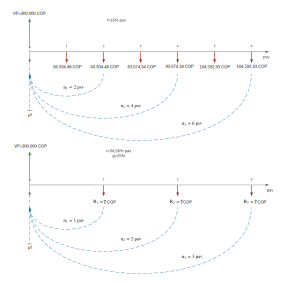
\includegraphics[trim=-78 -5 -78 -5]{7_Capitulo/img/ejemplos/8/8_3.pdf} }   \\ \hline
			%%%%% INICIO FLUJO DE CAJA
			\rowcolor[HTML]{FFB183}
			\multicolumn{2}{|c|}{\cellcolor[HTML]{FFB183}\textbf{4. Declaración de fórmulas}} \\ \hline
			%%%%%%%%%%%%% FIN INSERCIÓN DE IMAGEN
			%%%%%FIN FLUJO DE CAJA
		
			\multicolumn{2}{|c|}{ $VP = \frac{R( (1 + g)^{n} (1+i)^{-n} - 1)}{g-i} $ Valor presente gradiente geométrico}   \\  \hline
			
			%%%%%% INICIO DESARROLLO MATEMÁTICO
			\rowcolor[HTML]{FFB183}
			%%%%%%%%%%INICIO TITULO
			\multicolumn{2}{|c|}{\cellcolor[HTML]{FFB183}\textbf{5. Desarrollo matemático}}       \\ \hline
			%%%%%%%%%% FIN TITULO
			%%%%%%%%%% INICIO MATEMÁTICAS
			\multicolumn{2}{|c|}{  $300.000 \ COP = \frac{R_{1}( (1 + 0,25)^{3} (1+0,3456)^{-3} - 1)}{0,25-0,3456} $}   \\ 
			\multicolumn{2}{|c|}{ $ R_{1} = 225.920,73 \ COP $ }   \\ \hline
			
			%%%%%%%%%% FIN MATEMÁTICAS
			%%%%%% FIN DESARROLLO MATEMÁTICO
			%%%%%% INICIO RESPUESTA
			\rowcolor[HTML]{FFB183}
			%%%%%%%%%%INICIO TITULO
			\multicolumn{2}{|c|}{\cellcolor[HTML]{FFB183}\textbf{6. Respuesta}}   \\ \hline
			%%%%%%%%%% FIN TITULO
			%%%%%%%%%% INICIO RESPUESTA MATEMÁTICA
			\multicolumn{2}{|c|}{ 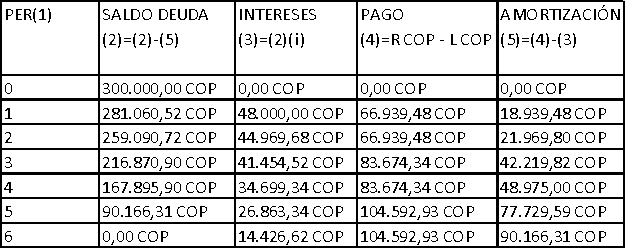
\includegraphics[trim=-78 -5 -78 -5]{7_Capitulo/img/ejemplos/8/8_3_3.pdf} }   \\ \hline
			%\multicolumn{2}{|C{\textwidth}|}{
			%	$R_{58} =  COP  72.478,16(1 + 0,02)^{57} =  COP  224.087,15 $ 
			%}  \\ \hline
			
			
			%%%%%%%%%% FIN MATEMÁTICAS
			%%%%%% FIN RESPUESTA
		\end{longtable}
		%Se crean dos lineas en blanco para que no quede el siguiente texto tan pegado
		%\newline \newline %USARLO SI CREES QUE ES NECESARIO
	\end{center}
 %%%%%%%%%%%%%%%%%%%%%%%%%%FIN EJERCICIO 8c %%%%%%%%%%%%%%%%%%%%%%%%%%%
    %%%%%%%%%%%%%%%%%%%%%%%%%%FIN EJERCICIO 8c %%%%%%%%%%%%%%%%%%%%%%%%%%%

%%%%%%%%%%%%%%%%%%%%%%%%%%FIN EJERCICIO 8 %%%%%%%%%%%%%%%%%%%%%%%%%%%
%%%%%%%%%%%%%%%%%%%%%%%%%%FIN EJERCICIO 8 %%%%%%%%%%%%%%%%%%%%%%%%%%%

%%%%%%%%%% NO OLVIDAR COLOCAR ESTE COMENTARIO CON EL NUMERO DE EJERCICIO %%%%%%%%%%%%%
%%%%%%%%%%%%%%%%%%% EJERCICIO 9 %%%%%%
%%Text bf para negrilla , el \\ es para el salto de linea.
%%El primer \\ hace un espacio en el texto y el 2 \\ crea otro espacio
\textbf{Ejemplo 7}\newline
Elaborar una tabla para amortizar la suma de 10.000.000 COP en 4 pagos iguales, suponiendo una tasa de interés de 40\% nominal anual trimestre vencido.\\ \\

\textbf{Solución.}\\
\begin{center}

    \renewcommand{\arraystretch}{1.5}% Margenes de las celdas
    %Creación de la cuadricula
    \begin{longtable}{|c|c|c| }
        %Creamos una linea horizontal
        \hline
        %Definimos el color de la primera fila
        \rowcolor[HTML]{FFB183}
        %%%%% INICIO ASIGNACIÓN FECHA FOCAL %%%%%%%
        %%%%%%%%%% INICIO TITULO
        %Lo que se hace aquí es mezclar las 3 columnas en una sola
        \multicolumn{3}{|c|}{\cellcolor[HTML]{FFB183}\textbf{1. Asignación período focal}}   \\ \hline
        %%%%%%%%%% FIN TITULO
        %%%%% INICIO DECLARACIÓN DE VARIABLES %%%%%%%
        \multicolumn{3}{|c|}{$pf = 0 ptv$} \\ \hline
        %Definimos el color de la primera fila
        \rowcolor[HTML]{FFB183}
        %%%%% INICIO DECLARACIÓN DE VARIABLES %%%%%%%
        %%%%%%%%%% INICIO TITULO
        \multicolumn{3}{|c|}{\cellcolor[HTML]{FFB183}\textbf{2. Declaración de variables}}      \\ \hline
        %%%%%%%%%% FIN TITULO
        %%%%%%%%%% INICIO DE MATEMÁTICAS
        \multicolumn{3}{|c|}{$j=40\% natv \equiv 10\% ptv =i$}\\ \hline
        $n=4$  ptv & $VP =$ 10.000.000 COP & $R= ? COP $                                                                     \\ \hline

        %%%%%%%%%% FIN DE MATEMÁTICAS
        %%%%% FIN DECLARACIÓN DE VARIABLES


        %%%%% INICIO FLUJO DE CAJA
        \rowcolor[HTML]{FFB183}
        \multicolumn{3}{|c|}{\cellcolor[HTML]{FFB183}\textbf{3. Diagrama de flujo de caja}}         \\ \hline
        %Mezclamos 3 columnas y pondremos el dibujo
        %%%%%%%%%%%%% INSERCIÓN DE LA IMAGEN
        \multicolumn{3}{|c|}{ \includegraphics[scale=1]{4_Capitulo/img/ejemplos/9/capitulo4ejemplo9.pdf} } \\ \hline 
        %%%%%%%%%%%%% FIN INSERCIÓN DE IMAGEN
        %%%%%FIN FLUJO DE CAJA



        %%%%% INICIO DECLARACIÓN FORMULAS
        %%%%%%%%%%% INICIO TITULO
        \rowcolor[HTML]{FFB183}
        \multicolumn{3}{|c|}{\cellcolor[HTML]{FFB183}\textbf{4. Declaración de fórmulas}}       \\ \hline
        %%%%%%%%%%% FIN TITULO
        %%%%%%%%%%% INICIO MATEMÁTICAS

        \multicolumn{3}{|c|}{$VP=R\frac{(1-(1+i)^{-n})}{i}$ Valor presente serie uniforme vencida}  \\ \hline
        %%%%%%%%%% FIN MATEMÁTICAS
        %%%%%% INICIO DESARROLLO MATEMÁTICO
        \rowcolor[HTML]{FFB183}
        %%%%%%%%%%INICIO TITULO
        \multicolumn{3}{|c|}{\cellcolor[HTML]{FFB183}\textbf{5. Desarrollo matemático}}    \\ \hline
        %%%%%%%%%% FIN TITULO
        %%%%%%%%%% INICIO MATEMÁTICAS
        \multicolumn{3}{|c|}{10.000.000 COP$=R\frac{(1-(1+0,1)^{-4})}{0,1}$ }     \\ \hline
        %%%%%%%%%% FIN MATEMÁTICAS
        %%%%%% FIN DESARROLLO MATEMÁTICO

        \rowcolor[HTML]{FFB183}
        \multicolumn{3}{|c|}{\cellcolor[HTML]{FFB183}\textbf{6. Respuesta}}    \\ \hline

        \multicolumn{3}{|c|}{R=3.154.708 COP} \\ \hline
        \multicolumn{3}{|c|}{ \includegraphics[scale=0.8]{4_Capitulo/img/ejemplos/9/Capitulo4Ejemplo9Solucion.pdf} } \\ \hline      
    \end{longtable}
    %Se crean dos lineas en blanco para que no quede el siguiente texto tan pegado
    %\newline \newline
\end{center}
%%%%%%%%%%%%%%%%%%%%%%%%%%FIN EJERCICIO X %%%%%%%%%%%%%%%%%%%%%%%%%%%


\newpage
	\textbf{Ejemplo 10}\newline
Supongamos que faltando 10 días para el vencimiento el inversionista del ejemplo anterior decide venderlo y para esta época se están negociando en Bolsa con una tasa del 28\% período 10 días vencido, por lo tanto la tasa de registro debe ser del 28\% período 10 días Vencido. El valor de compra del ejemplo anterior es de 97,204\% COP (faltando 40 días) Suponer el año de 365 días. Calcular:\\
1. El precio de registro en bolsa. \\
2. La retención en la fuente que debe reconocer al vendedor. \\
3. La tasa del vendedor. \\
4. El precio de vendedor. \\
5. Valor de venta.  \\
6. Tasa del comprador. \\
7. Valor del comprador. \newline
\textbf{Solución.
\newline}
\begin{center}
    \renewcommand{\arraystretch}{1.5}% Margenes de las celdas
    %Creación de la cuadricula
    \begin{longtable}[H]{|c|c|c| }
        %Creamos una linea horizontal
        \hline
        %Definimos el color de la primera fila
        \rowcolor[HTML]{FFB183}
        %%%%% INICIO ASIGNACIÓN FECHA FOCAL %%%%%%%
        %%%%%%%%%% INICIO TITULO
        %Lo que se hace aquí es mezclar las 3 columnas en una sola
        \multicolumn{3}{|c|}{\cellcolor[HTML]{FFB183}\textbf{1. Asignación período focal}}   \\ \hline
        %%%%%%%%%% FIN TITULO
        %%%%% INICIO DECLARACIÓN DE VARIABLES %%%%%%%
        \multicolumn{3}{|c|}{$pf = 10 pdv $} \\ \hline
        %Definimos el color de la primera fila
        \rowcolor[HTML]{FFB183}
        %%%%% INICIO DECLARACIÓN DE VARIABLES %%%%%%%
        %%%%%%%%%% INICIO TITULO
        \multicolumn{3}{|c|}{\cellcolor[HTML]{FFB183}\textbf{2. Declaración de variables}}                                                                                   \\ \hline
        %%%%%%%%%% FIN TITULO
        %%%%%%%%%% INICIO DE MATEMÁTICAS
        $F =  100 COP  $ & 
        \multicolumn{2}{c|}{$ a) P_{r} =  ? COP;$\hspace{0.5cm}$ b) i_{v} =  ? \% pdv $} \\
        $ n = 10/365 = 0,027 pdv $ &
        \multicolumn{2}{c|}{$ c) P_{v} = ? COP;$\hspace{0.5cm}$ d) V_{v} =  ? COP $} \\
        $ n = (40-10)/365 pdv $ &
        \multicolumn{2}{c|}{ $ e) i_{c} = ? \% pdv;$\hspace{0.5cm}$ f) P_{c} = ? COP $ } \\
        $ i_{r} = 28\% 10 pdv $     & 
        \multicolumn{2}{c|}{ $ g) V_{c} = ? COP;$\hspace{0.5cm}$ h) R_{F} = ? COP $ } \\
        $ P_{c1} =  97,204 COP $   & 
        \multicolumn{2}{c|}{ $  $ }
        \\ \hline
        %%%%%%%%%% FIN DE MATEMÁTICAS
        %%%%% FIN DECLARACIÓN DE VARIABLES
        
        
        %%%%% INICIO FLUJO DE CAJA
        \rowcolor[HTML]{FFB183}
        \multicolumn{3}{|c|}{\cellcolor[HTML]{FFB183}\textbf{3. Diagrama de flujo de caja}}                                                                                  \\ \hline
        %Mezclamos 3 columnas y pondremos el dibujo
        %%%%%%%%%%%%% INSERCIÓN DE LA IMAGEN
\multicolumn{2}{|c|}{ 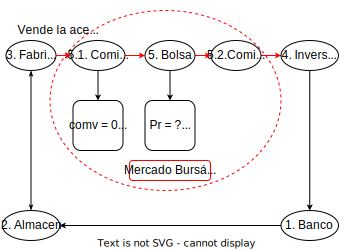
\includegraphics[trim=-90 -5 -90 -5]{3_Capitulo/img/ejemplos/10/capitulo3ejercicio10.pdf} }                                                                                      \\ \hline
        %%%%%%%%%%%%% FIN INSERCIÓN DE IMAGEN
        %%%%%FIN FLUJO DE CAJA
        
        
        
        %%%%% INICIO DECLARACIÓN FORMULAS
        %%%%%%%%%%% INICIO TITULO
        \rowcolor[HTML]{FFB183}
        \multicolumn{3}{|c|}{\cellcolor[HTML]{FFB183}\textbf{4. Declaración de fórmulas}}                                                                                    \\ \hline
        %%%%%%%%%%% FIN TITULO
        %%%%%%%%%%% INICIO MATEMÁTICAS
    
         \multicolumn{3}{|c|}{$P=F(1+i)^{-n}$\hspace{35pt}\textit{Valor presente}
         \hspace{0.3cm}}\\
         \multicolumn{3}{|c|}{$R_{F} = (F - P)*0,7$\hspace{35pt}\textit{Retención en la fuente}
         \hspace{0.3cm}}\\
         \multicolumn{3}{|c|}{$V_{V} = P_{V} * V_{total}$\hspace{35pt}\textit{}
         \hspace{0.3cm}}\\
         \multicolumn{3}{|c|}{$V_{C} = P_{C} * V_{total}$\hspace{35pt}\textit{}
         \hspace{0.3cm}}\\
        
         
         \hline
        %%%%%%%%%% FIN MATEMÁTICAS
        %%%%%% INICIO DESARROLLO MATEMÁTICO
        \rowcolor[HTML]{FFB183}
        %%%%%%%%%%INICIO TITULO
        \multicolumn{3}{|c|}{\cellcolor[HTML]{FFB183}\textbf{5. Desarrollo matemático}}                                                                                      \\ \hline
        %%%%%%%%%% FIN TITULO
        %%%%%%%%%% INICIO MATEMÁTICAS
         \multicolumn{3}{|c|}{$ a) P_{r} = 100 COP * (1 + 0,28)^{-10/365} = 99,3260\% COP$
         \hspace{0.3cm}}\\
         \multicolumn{3}{|c|}{$ b) 97,204 COP = 99.3260 (1+i)^{-30/365} => i_{v} = 6,4\% pdv$
         \hspace{0.3cm}}\\
         \multicolumn{3}{|c|}{$ d) V_{v} = 0,972 COP * 5{.}000{.}000 COP = 4{.}860{.}000 COP $
         \hspace{0.3cm}}\\
         \multicolumn{3}{|c|}{$ e) 99,3260 \% = 100 COP (1+ i)^{-10/365} => i = 9,84\%$
         \hspace{0.3cm}}\\
         \multicolumn{3}{|c|}{$ f) P_{c} = 100 COP (1 + 0,0984)^{-10/365} = 90,16\% COP $
         \hspace{0.3cm}}\\
         \multicolumn{3}{|c|}{$ g) V_{c} = 0,9016 * 5{.}000{.}000 COP = 4{.}508{.}000 COP $
         \hspace{0.3cm}}\\
         \multicolumn{3}{|c|}{$ h) R_{F} = 0,07(5{.}000{.}000 - 97,204) $
         \hspace{0.3cm}}\\
         
        %%%%%%%%%% FIN MATEMÁTICAS
        %%%%%% FIN DESARROLLO MATEMÁTICO
        
        \rowcolor[HTML]{FFB183}
        \multicolumn{3}{|c|}{\cellcolor[HTML]{FFB183}\textbf{6. Respuesta}} \\ \hline    
        
        \multicolumn{3}{|c|}{$P_{r} = 4{.}964{.}190 COP $} \\ \hline
    \end{longtable}
    %Se crean dos lineas en blanco para que no quede el siguiente texto tan pegado
\end{center}


\textbf{Ejemplo 11}\\
Se hacen depósitos trimestrales con incremento del 5\% entre flujos, en una cuenta que paga el 5,25\% periódica trimestral vencida, con el fin de tener disponibles 500.000 COP el primero de enero de 1991, Si el primer depósito se hace el primero de abril de 1988 y el último el primero de julio de 1990, determinar el valor del primer depósito:\\

	%%%%%%%%%%%%%%%%%%% EJERCICIO 11 %%%%%%

%\newpage %USAR SOLO SI EL SOLUCIÓN QUEDA SOLO Y ES NECESARIO BAJARLO A LA SIGUIENTE PAGINA
\textbf{Solución.}\\
%La tabla ira centrada
\begin{center}
	\renewcommand{\arraystretch}{1.6}% Margenes de las celdas
	%Creación de la cuadricula de 3 columnas
	\begin{longtable}[H]{|c|c|c|}
		%Creamos una linea horizontal
		\hline
		%Definimos el color de la primera fila
		\rowcolor[HTML]{FFB183}
		%%%%% INICIO ASIGNACIÓN FECHA FOCAL %%%%%%%
		%%%%%%%%%% INICIO TITULO
		%Lo que se hace aquí es mezclar las 3 columnas en una sola
		\multicolumn{3}{|c|}{\cellcolor[HTML]{FFB183}\textbf{1. Asignación período focal}}  \\ \hline
		\multicolumn{3}{|c|}{$pf = \textit{12 ptv}$}   \\\hline
		%%%%%%%%%% FIN TITULO
		%%%%% INICIO DECLARACIÓN DE VARIABLES %%%%%%%
		%%%%%%%%%% INICIO TITULO
		%Lo que se hace aquí es mezclar las 3 columnas en una sola
		\multicolumn{3}{|c|}{\cellcolor[HTML]{FFB183}\textbf{2. Declaración de variables}}   \\ \hline
		%%%%%%%%%% FIN TITULO
		%%%%%%%%%% INICIO DE MATEMÁTICAS
		%Cada & hace referencia al paso de la siguiente columna
		\multicolumn{2}{|c|}{$\hspace{2 cm}VP=  500{.}000 COP \hspace{2 cm}$} & $i=5.25\% \textit{ ptv}$ \\
		\multicolumn{2}{|c|}{$\hspace{2 cm}n_1=10  \textit{ pav} \hspace{2 cm}$} & $g=5\% \textit{crecimiento geométrico periódico } $ \\
		\multicolumn{2}{|c|}{$\hspace{2 cm}n_2=2  \textit{ pav} \hspace{2 cm}$} & $R= ?COP $ \\ \hline	
		
		%%%%%%%%%% FIN DE MATEMÁTICAS
		%%%%% FIN DECLARACIÓN DE VARIABLES
		
		%%%%% INICIO FLUJO DE CAJA
		\rowcolor[HTML]{FFB183}
		\multicolumn{3}{|c|}{\cellcolor[HTML]{FFB183}\textbf{3. Diagrama de flujo de caja}} \\ \hline
		%Mezclamos 3 columnas y pondremos el dibujo
		%%%%%%%%%%%%% INSERCIÓN DE LA IMAGEN
		%Deberán descargar las imágenes respectivas del drive y pegarlas en la carpeta
		%n_capitulo/img/ejemplos/1/capitulo1ejemplo1.pdf  (el /1/ es el numero del ejemplo)
		\multicolumn{3}{|c|}{ \includegraphics[trim=-5 -5 -5 -5 , scale=0.8]{6_Capitulo/img/ejemplos/11/Capitulo6Ejemplo11.pdf} }
		\\ \hline
		%%%%%%%%%%%%% FIN INSERCIÓN DE IMAGEN
		%%%%%FIN FLUJO DE CAJA
		
		%%%%% INICIO DECLARACIÓN FORMULAS
		%%%%%%%%%%% INICIO TITULO
		\rowcolor[HTML]{FFB183}
		\multicolumn{3}{|c|}{\cellcolor[HTML]{FFB183}\textbf{4. Declaración de fórmulas}}    \\ \hline
		%%%%%%%%%%% FIN TITULO
		%%%%%%%%%%% INICIO MATEMÁTICAS
		\multicolumn{3}{|c|}{$VF=(\frac{(R)[(1+g)^{n}-(1+i)^{n}]}{g-i}) \hspace{0.4 cm} \textit{Valor futuro gradiente si } g \neq i $} \\  
		\multicolumn{3}{|c|}{$F=P(1+i)^{n} \hspace{0.4 cm} \textit{Valor futuro}$} \\ \hline
		
		%%%%%%%%%% FIN MATEMÁTICAS
		%%%%%% INICIO DESARROLLO MATEMÁTICO
		\rowcolor[HTML]{FFB183}
		%%%%%%%%%%INICIO TITULO
		\multicolumn{3}{|c|}{\cellcolor[HTML]{FFB183}\textbf{5. Desarrollo matemático}}       \\ \hline
		%%%%%%%%%% FIN TITULO
		%%%%%%%%%% INICIO MATEMÁTICAS
		\multicolumn{3}{|c|}{$ 500{.}000COP=\frac{(R)[(1-0.05)^{10}-(1+0.0525)^{-10}]}{0.5-0.0525} \cdot (1+0.0525)^{2}  \hspace{0.4 cm} $} \\ \hline
		%%%%%%%%%% FIN MATEMÁTICAS
		%%%%%% FIN DESARROLLO MATEMÁTICO
		%%%%%% INICIO RESPUESTA
		\rowcolor[HTML]{FFB183}
		%%%%%%%%%%INICIO TITULO
		\multicolumn{3}{|c|}{\cellcolor[HTML]{FFB183}\textbf{6. Respuesta}}   \\ \hline
		%%%%%%%%%% FIN TITULO
		%%%%%%%%%% INICIO RESPUESTA MATEMÁTICA
		\multicolumn{3}{|c|}{${R=  72{.}468.80COP}$} \\ \hline
		%%%%%%%%%% FIN MATEMÁTICAS
		%%%%%% FIN RESPUESTA
	\end{longtable}
	%Se crean dos lineas en blanco para que no quede el siguiente texto tan pegado
	%\newline \newline %USARLO SI CREES QUE ES NECESARIO
\end{center}

%%%%%%%%%%%%%%%%%%%%%%%%%%FIN EJERCICIO 11 %%%%%%%%%%%%%%%%%%%%%%%%%%%

%\textbf{Ejemplo 9}\\
%Supongamos que un inversionista desea adquirir la aceptación bancaria del ejemplo anterior, la cual figura con una tasa de registro del 30\% periódico 40 días vencido y con precio de registro $P_{R} =  COP 97,165$ pero él también sabe que para adquirirla deberá pagar una comisión a un corredor de bolsa lo cual hará variar el precio que él debe pagar y también la rentabilidad que él pueda obtener.\\
%
%Supongamos que la comisión que cobra un corredor por la compra es del 0,475\% periodo 40 días periodo vencido\\
%¿Cuál es el precio del inversionista?$ P_{c} =  COP ? $, que incluye la comisión del comisionista vendedor, el precio de registro y la comisión de bolsa del comprador. El punto de referencia es el precio de registro $P_{R}$.\\
%¿Cuál es la rentabilidad del inversionista? $i_{c} = ? \%$ periódica 40 días vencido, o $j =? nadv$
%
%\textbf{Solución}\\
%\begin{itemize}
%  \item a. Diagrama de flujo\\
%        \begin{center}
%          \includegraphics[height=6.0cm]{3_Capitulo/img/ejemplos/3_10}
%        \end{center}
%  \item b. Declaración de variables\\
%        $i_{c} = 30\% - 0,475\% = 29,525\% p 40dv\\
%          P_c =  COP ?$\\
%        $n= \frac{40}{365} p (40días) $\\
%        $P_{R}=?$\\
%  \item c.Declaración de formulas\\
%        \\
%        P = $F(1+i)^{n}$ \hspace{35pt}\textit{Valor presente}\\
%  \item d. Desarrollo matemático:\\
%        \\
%        $P_c =   COP 100(1+0,29525)^\frac{40}{365} =  COP 97,2047$ \hspace{35pt}\textit{Ecuación de valor} \\
%        $P_{R}$ =  COP 97,2047\% ( COP 5{.}000{.}000) =  COP 4{.}860,245\\
%        $P_c-P_{R}$ =  COP 4{.}860,235 -  COP 4{.}858,285 =  COP 1{.}950\\
%  \item e. Respuesta\\
%        \\
%        Precio del Inversionista =  COP  97,2047 y la rentabilidad inversionista fue de 29,52\% p(40dv) \\
%
%
%\end{itemize}
%\textbf{Observación:} En el mercado bursátil el precio del vendedor es diferente al precio del comprador debido a la comisión de los corredores de bolsa, pero en el mercado extrabursátil estos valores son iguales dado que no hay comisión.\\
%
%En el ejemplo anterior hemos mostrado el procedimiento de negociación en los mercados extra bursátil y bursátil, pero por simplicidad no hemos incluido el impuesto y la comisión que cobra el banco por la expedición de la aceptación bancaria. En el siguiente ejemplo incluiremos este factor.\\
%\textbf{Ejercicio 10}\\
%
%Supongamos que faltando 10 días para el vencimiento el inversionista del ejemplo anterior decide venderlo y para esta época se están negociando en Bolsa con una tasa del 28\% período 10 días vencido, por lo tanto la tasa de registro debe ser del 28\% período 10 días Vencido. \\
%Calcular: \\
%El precio de registro en bolsa. \\
%La retención en la fuente que debe reconocer al vendedor. \\
%La tasa del vendedor. \\
%El precio de vendedor. \\
%Valor de venta.  \\
%Tasa del comprador. \\
%Valor del comprador. \\
%\begin{itemize}
%  \item a.Diagrama de flujo:\\
%
%  \item b.Declaración de variables
%
%        F =  COP 100\\ i= 28\% p(10d)v  COP n= \frac{10}{365}$p(10d)v\\
%        Pr =  COP ?\\
%  \item d.Declaración de formulas:\
%
%        $P=F(1+i    )^{-n}$\hspace{35pt}\textit{Valor presente}\\
%
%  \item e. Desarrollo matemático
%
%        $P_{R}= COP 100 (1+0,28)^\frac{-10}{365}$ = 99,32595\% \hspace{35pt}\textit{Ecuación de valor}\\
%
%        En pesos el valor de registro será: 99,3595\% x  COP 5{.}000{.}000 =  COP 4{.}966,298\\
%        Por lo tanto, la retención en la fuente será RF = 0,07*( COP 5{.}000{.}000 -  COP 4{.}966,298) =  COP 2{.}359\\
%        Suponiendo que las comisiones de compra y venta sean c/u del 0,5\% en rentabilidad la tasa del vendedor viene a ser 28\% + 0,5\% = 28,5\% período 10 días vencido y el precio de venta será:
%        \begin{center}
%          $	P_{V} = 100(1+0,285)^\frac{-10}{365}$ = 99,3153\% equivalente a 99,3153\%(  COP 5{.}000{.}000) =  COP 4{.}965,765\\
%        \end{center}
%        Por lo tanto el vendedor además de recibir los  COP 4{.}965{.}765 también debe recibir lo correspondiente a la retención en la fuente ( COP 2,359), En consecuencia el vendedor recibirá:\\
%        \begin{center}
%          $P_{V}$ =  COP 4{.}966{.}830 +  COP 2{.}539 =  COP 4{.}969{.}189
%        \end{center}
%        Para el comprador se tiene:
%        \begin{center}
%          Tasa de compra ic = 28\% - 0,5\% = 27,5\% p10dv
%        \end{center}
%        Precio de compra:
%        \begin{center}
%          Pc = $100(1+0,275)^\frac{-10}{365}$ = 99,3366\% equivalente a 99,3366\% x  COP 5{.}000{.}000 =  COP 4{.}966{.}830
%        \end{center}
%        El total que debe pagar el comprador será el precio de compra más la parte de retención en la fuente que la Bolsa le devuelve al vendedor, esto es:
%        \begin{center}
%          Pc Neto= 	 COP 4{.}966{.}830 +  COP 2{.}359 =  COP 4{.}969{.}189
%        \end{center}
%  \item e. Respuesta\\
%        \textbf{Observación 1:} El primer inversionista pagó por retención en la fuente  COP 9{.}920 y le reintegraron  COP 2{.}359 esto significa que en total pagó:  COP 9{.}920- COP 2{.}359	=  COP 7{.}561 y el segundo inversionista pagó  COP 2{.}359\\
%        \textbf{Observación 2:} La constitución de aceptaciones no implica desembolsos de dinero en forma inmediata ni por parte de la entidad financiera ni por parte del comprador, salvo el IVA de la mercancía,  la comisión de intermediario financiero, lo demás es una obligación futura.\\
%        \textbf{Observación 3:} Si una aceptación no es cobrada al vencimiento, el emisor debe consignar el valor de esta en el Banco Agrario, sin embargo el emisor da un período de gracia antes de hacer la correspondiente consignación.
%\end{itemize}
%\medskip
%
%\textbf{Ejemplo 11}\\
%
%Una aceptación bancaria por  COP 80 millones con fecha de vencimiento el 17 de diciembre de 1999 es adquirida en 22 de julio de 1999 por un primer inversionista con una tasa del de 28\% período 28 días vencidos y es cedida a un segundo inversionista el 14 de octubre de 1999. Si el segundo inversionista desea ganarse el 32\% período días vencido utilice un año de 360 (año de 360 días) \\
%¿Cuál es la ganancia en pesos del primer inversionista? \\
%¿cuál es la rentabilidad periódica días vencido del primer inversionista? \\
%
%Si tomamos en cuenta que debemos usar un año de 360 días entonces los días que hay entre el 22 de julio y el 17 de diciembre son 145 que se calculan así: \\
%
%\begin{center}
%  \includegraphics[height=5.0cm]{3_Capitulo/img/ejemplos/3_12}
%\end{center}
%
%Los días que hay entre el 14 de octubre y el 17 de diciembre se calculan así:
%
%
%\begin{center}
%  \includegraphics[height=3.0cm]{3_Capitulo/img/ejemplos/3_13}
%\end{center}
%
%\textbf{Solución}\\
%\begin{itemize}
%  \item a. Diagrama de flujo\\
%        \begin{center}
%          \includegraphics[height=4.0cm]{3_Capitulo/img/ejemplos/3_14}
%        \end{center}
%  \item b. Declaración de variables\\
%        $i_{1} = 28\% pav$ \\
%        $n_{1} = \frac{145}{360}$ pav\\
%        $i_{2} = 32 \%$ pdv\\
%        $n_{2} =\frac{63}{360}$pdv\\
%        $n_{3} = 145$ días - 63 días = 82 pdv.\\
%
%        $P_{c2}-P_{c1} = ?$\\\\
%
%  \item c. Declaración de formulas\\
%
%        P = $F(1+i)^{-n}$ \hspace{35pt}\textit{Valor presente}\\
%
%  \item d. Desarrollo matemático\\
%        $Pc_1 =  COP 80{.}000{.}000(1+0,28)\frac{-145}{360}$ =  COP  72{.}428{.}283,64 $\simeq$  COP 72{.}428{.}284 \hspace{35pt}\textit{Ecuación de valor}\\
%        $Pc_2 =  COP 80{.}000{.}000(1+0,32)\frac{-63}{360}$ =  COP  76{.}206{.}067,12\\
%  \item e. Respuesta:\\
%        La ganancia del primer inversionista será:\\
%        \begin{center}
%          $Pc_2 - Pc_1 =  COP 76{.}206{.}067 -  COP 72{.}428{.}284 =  COP 3{.}777{.}783$\\
%        \end{center}
%\end{itemize}
%En este caso el tiempo se puede hallar calculando los días que hay entre el 22 de julio y el 14 de octubre usando el procedimiento anterior, o, también por diferencia de días entre el total que es 145 y los que hay entre la fecha de compra del segundo inversionista y a la fecha de vencimiento que vienen a ser 63 días, entonces esta diferencia viene a ser: 145 - 63 = 82
%\begin{center}
%   COP 76{.}206{.}067 = $ COP 72{.}428{.}284(1+i)\frac{82}{360}$
%\end{center}
%De donde se obtiene que i= 25,01\%\ período 82 días vencidos \\
%La rentabilidad del segundo inversionista obviamente es del 32\% periodo (63 días vencidos).
%\chapter{Modelos de Conteo}

%\section{Introducción}\index{Introducción}



%----------------------------------------------------------------------------------------
%	PART
%----------------------------------------------------------------------------------------

%\part{Parte Dos}

%----------------------------------------------------------------------------------------
%	CHAPTER 3
%----------------------------------------------------------------------------------------

%\chapterimage{ima2} % Chapter heading image


%Anexos
%\chapter*{Anexos}
%\addcontentsline{toc}{chapter}{\textcolor{ocre}{Anexos}}




%----------------

%----------------------------------------------------------------------------------------
%	BIBLIOGRAPHY
%----------------------------------------------------------------------------------------

%\chapter*{Bibliografía}
%\addcontentsline{toc}{chapter}{\textcolor{ocre}{Bibliografía}}
%\section*{Books}
%\addcontentsline{toc}{section}{Books}
%\printbibliography[heading=bibempty,type=book]

%\begin{itemize}
%\item


%\end{itemize}


%----------------------------------------------------------------------------------------
%	INDEX
%----------------------------------------------------------------------------------------

\phantomsection
\setlength{\columnsep}{0.75cm}
\printindex
